% Options for packages loaded elsewhere
\PassOptionsToPackage{unicode}{hyperref}
\PassOptionsToPackage{hyphens}{url}
%
\documentclass[
]{article}
\usepackage{amsmath,amssymb}
\usepackage{iftex}
\ifPDFTeX
  \usepackage[T1]{fontenc}
  \usepackage[utf8]{inputenc}
  \usepackage{textcomp} % provide euro and other symbols
\else % if luatex or xetex
  \usepackage{unicode-math} % this also loads fontspec
  \defaultfontfeatures{Scale=MatchLowercase}
  \defaultfontfeatures[\rmfamily]{Ligatures=TeX,Scale=1}
\fi
\usepackage{lmodern}
\ifPDFTeX\else
  % xetex/luatex font selection
\fi
% Use upquote if available, for straight quotes in verbatim environments
\IfFileExists{upquote.sty}{\usepackage{upquote}}{}
\IfFileExists{microtype.sty}{% use microtype if available
  \usepackage[]{microtype}
  \UseMicrotypeSet[protrusion]{basicmath} % disable protrusion for tt fonts
}{}
\makeatletter
\@ifundefined{KOMAClassName}{% if non-KOMA class
  \IfFileExists{parskip.sty}{%
    \usepackage{parskip}
  }{% else
    \setlength{\parindent}{0pt}
    \setlength{\parskip}{6pt plus 2pt minus 1pt}}
}{% if KOMA class
  \KOMAoptions{parskip=half}}
\makeatother
\usepackage{xcolor}
\usepackage[margin=1in]{geometry}
\usepackage{color}
\usepackage{fancyvrb}
\newcommand{\VerbBar}{|}
\newcommand{\VERB}{\Verb[commandchars=\\\{\}]}
\DefineVerbatimEnvironment{Highlighting}{Verbatim}{commandchars=\\\{\}}
% Add ',fontsize=\small' for more characters per line
\usepackage{framed}
\definecolor{shadecolor}{RGB}{248,248,248}
\newenvironment{Shaded}{\begin{snugshade}}{\end{snugshade}}
\newcommand{\AlertTok}[1]{\textcolor[rgb]{0.94,0.16,0.16}{#1}}
\newcommand{\AnnotationTok}[1]{\textcolor[rgb]{0.56,0.35,0.01}{\textbf{\textit{#1}}}}
\newcommand{\AttributeTok}[1]{\textcolor[rgb]{0.13,0.29,0.53}{#1}}
\newcommand{\BaseNTok}[1]{\textcolor[rgb]{0.00,0.00,0.81}{#1}}
\newcommand{\BuiltInTok}[1]{#1}
\newcommand{\CharTok}[1]{\textcolor[rgb]{0.31,0.60,0.02}{#1}}
\newcommand{\CommentTok}[1]{\textcolor[rgb]{0.56,0.35,0.01}{\textit{#1}}}
\newcommand{\CommentVarTok}[1]{\textcolor[rgb]{0.56,0.35,0.01}{\textbf{\textit{#1}}}}
\newcommand{\ConstantTok}[1]{\textcolor[rgb]{0.56,0.35,0.01}{#1}}
\newcommand{\ControlFlowTok}[1]{\textcolor[rgb]{0.13,0.29,0.53}{\textbf{#1}}}
\newcommand{\DataTypeTok}[1]{\textcolor[rgb]{0.13,0.29,0.53}{#1}}
\newcommand{\DecValTok}[1]{\textcolor[rgb]{0.00,0.00,0.81}{#1}}
\newcommand{\DocumentationTok}[1]{\textcolor[rgb]{0.56,0.35,0.01}{\textbf{\textit{#1}}}}
\newcommand{\ErrorTok}[1]{\textcolor[rgb]{0.64,0.00,0.00}{\textbf{#1}}}
\newcommand{\ExtensionTok}[1]{#1}
\newcommand{\FloatTok}[1]{\textcolor[rgb]{0.00,0.00,0.81}{#1}}
\newcommand{\FunctionTok}[1]{\textcolor[rgb]{0.13,0.29,0.53}{\textbf{#1}}}
\newcommand{\ImportTok}[1]{#1}
\newcommand{\InformationTok}[1]{\textcolor[rgb]{0.56,0.35,0.01}{\textbf{\textit{#1}}}}
\newcommand{\KeywordTok}[1]{\textcolor[rgb]{0.13,0.29,0.53}{\textbf{#1}}}
\newcommand{\NormalTok}[1]{#1}
\newcommand{\OperatorTok}[1]{\textcolor[rgb]{0.81,0.36,0.00}{\textbf{#1}}}
\newcommand{\OtherTok}[1]{\textcolor[rgb]{0.56,0.35,0.01}{#1}}
\newcommand{\PreprocessorTok}[1]{\textcolor[rgb]{0.56,0.35,0.01}{\textit{#1}}}
\newcommand{\RegionMarkerTok}[1]{#1}
\newcommand{\SpecialCharTok}[1]{\textcolor[rgb]{0.81,0.36,0.00}{\textbf{#1}}}
\newcommand{\SpecialStringTok}[1]{\textcolor[rgb]{0.31,0.60,0.02}{#1}}
\newcommand{\StringTok}[1]{\textcolor[rgb]{0.31,0.60,0.02}{#1}}
\newcommand{\VariableTok}[1]{\textcolor[rgb]{0.00,0.00,0.00}{#1}}
\newcommand{\VerbatimStringTok}[1]{\textcolor[rgb]{0.31,0.60,0.02}{#1}}
\newcommand{\WarningTok}[1]{\textcolor[rgb]{0.56,0.35,0.01}{\textbf{\textit{#1}}}}
\usepackage{longtable,booktabs,array}
\usepackage{calc} % for calculating minipage widths
% Correct order of tables after \paragraph or \subparagraph
\usepackage{etoolbox}
\makeatletter
\patchcmd\longtable{\par}{\if@noskipsec\mbox{}\fi\par}{}{}
\makeatother
% Allow footnotes in longtable head/foot
\IfFileExists{footnotehyper.sty}{\usepackage{footnotehyper}}{\usepackage{footnote}}
\makesavenoteenv{longtable}
\usepackage{graphicx}
\makeatletter
\def\maxwidth{\ifdim\Gin@nat@width>\linewidth\linewidth\else\Gin@nat@width\fi}
\def\maxheight{\ifdim\Gin@nat@height>\textheight\textheight\else\Gin@nat@height\fi}
\makeatother
% Scale images if necessary, so that they will not overflow the page
% margins by default, and it is still possible to overwrite the defaults
% using explicit options in \includegraphics[width, height, ...]{}
\setkeys{Gin}{width=\maxwidth,height=\maxheight,keepaspectratio}
% Set default figure placement to htbp
\makeatletter
\def\fps@figure{htbp}
\makeatother
\setlength{\emergencystretch}{3em} % prevent overfull lines
\providecommand{\tightlist}{%
  \setlength{\itemsep}{0pt}\setlength{\parskip}{0pt}}
\setcounter{secnumdepth}{5}
\usepackage{pdfpages}
\usepackage{graphicx}
\usepackage{tocloft}
\usepackage{xcolor}
\usepackage{tcolorbox}
\definecolor{myblue}{RGB}{0, 102, 204}
\tcbset{colback=myblue!20!white,colframe=myblue!75!black}
\usepackage{fancyhdr}
\usepackage{booktabs}
\usepackage{caption}
\usepackage{longtable}
\usepackage{colortbl}
\usepackage{array}
\ifLuaTeX
  \usepackage{selnolig}  % disable illegal ligatures
\fi
\IfFileExists{bookmark.sty}{\usepackage{bookmark}}{\usepackage{hyperref}}
\IfFileExists{xurl.sty}{\usepackage{xurl}}{} % add URL line breaks if available
\urlstyle{same}
\hypersetup{
  hidelinks,
  pdfcreator={LaTeX via pandoc}}

\title{\begin{center}\begin{tcolorbox}[colback=myblue!20!white,colframe=myblue!75!black,title={\textcolor{white}{\centering\bfseries Projet- logiciel statistique R: Le package gtsumary}}]\end{tcolorbox}\end{center}}
\author{``Groupe 12: ADAM Alassane, CISSE Pape Abdourahmane, NGOM
Fallou, YAMIN Youdan''}
\date{Dernière mise à jour: 26-mai-2024}

\begin{document}
\maketitle

\pagestyle{fancy}
\fancyhf{}
\fancyhead[L]{Projet- logiciel statistique R: Le package gtsumary}
\fancyfoot[C]{ADAM, CISSE, NGOM, KOLAMBIGUE}
\fancyfoot[R]{\thepage}

\maketitle

\includepdf{page_garde}
\newpage
\tableofcontents
\newpage

\begin{tcolorbox}[colback=red!5!white,colframe=black,title=Note,sharp corners]
La bibliothèque GTsummary est une puissante extension de R pour la création de tableaux de synthèse des résultats d'analyses statistiques. Son objectif principal est de simplifier et d'améliorer la création de rapports statistiques en fournissant des outils conviviaux pour résumer et présenter les résultats de manière claire et concise.

Pour utiliser gtsumary: Importer les données dans R, Utiliser les fonctions gtsummary pour résumer les resultats des analyses statistiques, personnaliser les tableaux générés selon vos besoins en utilisant les options de personnalisations disponibles, Intégrer les tableaux dans vos rapports ou présentations pour une communication claire et efficace des résultats.


\end{tcolorbox}

\hypertarget{i-pruxe9liminaires}{%
\section{I Préliminaires}\label{i-pruxe9liminaires}}

\hypertarget{i-1-utilituxe9}{%
\subsection{I-1 Utilité}\label{i-1-utilituxe9}}

Le package \texttt{gtsummary} en R est un outil puissant conçu pour la
génération de tableaux de synthèse de données statistiques de manière
élégante, personnalisable, reproductible et directement publiables. Il
intègre :

\begin{itemize}
\item
  \textbf{Tableaux descriptifs} : univariés, bivariés et de regression
\item
  \textbf{Résumés des données descriptives} : moyennes, médianes,
  écarts-types, fréquence \ldots{}
\item
  \textbf{Test statistiques} : t-test, khi-2\ldots{}
\item
  \textbf{Personnalisation avancé} : apparence, titres, légendes,
  annotations \ldots{}
\item
  \textbf{Reproductibilité} : Automatisation
\end{itemize}

\hypertarget{i-2-installation-et-types-de-variables}{%
\subsection{I-2 Installation et types de
variables}\label{i-2-installation-et-types-de-variables}}

\hypertarget{i-2-1-installation}{%
\subsubsection{I-2-1 Installation}\label{i-2-1-installation}}

\begin{itemize}
\tightlist
\item
  Installer depuis le CRAN :
\end{itemize}

\begin{Shaded}
\begin{Highlighting}[]
  \FunctionTok{install.packages}\NormalTok{(}\StringTok{"gtsummary"}\NormalTok{)}
\end{Highlighting}
\end{Shaded}

\begin{itemize}
\tightlist
\item
  Installer la version de dévellopement depuis github
\end{itemize}

\begin{Shaded}
\begin{Highlighting}[]
\NormalTok{remotes}\SpecialCharTok{::}\FunctionTok{install\_github}\NormalTok{(}\StringTok{"ddsjoberg/gtsummary"}\NormalTok{)}
\end{Highlighting}
\end{Shaded}

\hypertarget{i-2-2-types-de-variables}{%
\subsubsection{I-2-2 Types de
variables}\label{i-2-2-types-de-variables}}

Il y'a trois types de variables dans gtsummary. Par défaut, gtsummary
considère qu'une variable est :

\begin{itemize}
\item
  \textbf{Dichotomique} : s'il s'agit d'un vecteur logique (TRUE/FALSE),
  d'une variable textuelle codée yes/no ou d'une variable numérique
  codée 0/1.
\item
  \textbf{Catégorielle} : S'il s'agit d'un facteur, d'une variable
  textuelle ou d'une variable numérique ayant moins de 10 valeurs
  différentes.
\item
  \textbf{Continue} : Dans les autres cas de variables numériques.
\end{itemize}

\hypertarget{i-3-description-de-la-base-de-donnuxe9es}{%
\subsection{I-3 Description de la base de
données}\label{i-3-description-de-la-base-de-donnuxe9es}}

\begin{itemize}
\tightlist
\item
  \textbf{Source} : EHCVM 2018
\item
  \textbf{Taille} : 66120 ménages enquêtés et 11 variables
\item
  \textbf{Description} : Les variables renseignent sur la localisation
  des ménages, les carctérisques sociodémographiques du chef de ménage,
  la consommation annulle et les indicateurs de pauvreté.
\end{itemize}

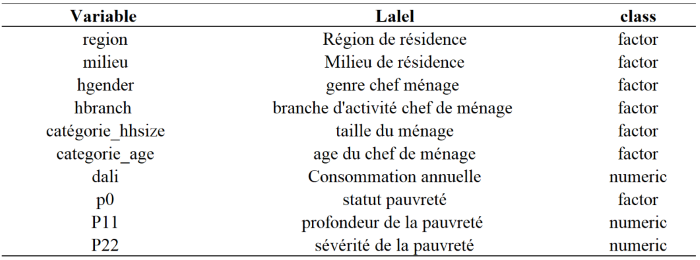
\includegraphics[width=9.72in]{../img/liste_var_}

\hypertarget{ii-tableau-descriptif-univariuxe9}{%
\section{II Tableau descriptif
univarié}\label{ii-tableau-descriptif-univariuxe9}}

\hypertarget{ii-1-thuxe9mes-du-tableaux}{%
\subsection{II-1 Thémes du tableaux}\label{ii-1-thuxe9mes-du-tableaux}}

gtsummary fournit plusieurs fonctions préfixées
\textbf{theme\_gtsummary()} permettent de modifier l'affichage par
défaut des tableaux. Parmis les Exemples de fonctions nous avons: La
fonction \textbf{theme\_gtsummary\_language}(Permets de modifier la
langue utlisés dans le tableaux), La fonction
\textbf{theme\_gtsummary\_journal}(Pour définir un thème prédéfini), La
fonction \textbf{reset\_gtsummary\_theme}(Pour effacer tous les thémes
précédemment définis)

\begin{Shaded}
\begin{Highlighting}[]
\CommentTok{\#Ramener le format du tableau en français }
\FunctionTok{theme\_gtsummary\_language}\NormalTok{(}\AttributeTok{language =} \StringTok{"fr"}\NormalTok{, }\AttributeTok{decimal.mark =} \StringTok{","}\NormalTok{,}
                         \AttributeTok{big.mark =} \StringTok{" "}\NormalTok{)}
\end{Highlighting}
\end{Shaded}

\hypertarget{ii-2-la-fonction-tbl_summary}{%
\subsection{II-2 La fonction
tbl\_summary}\label{ii-2-la-fonction-tbl_summary}}

La fonction au coeur du package \textbf{gtsummary} se nomme
\textbf{tbl\_summary()}.Elle produit un tableau qui s'affiche dans
l'onglet ``Viewer''. On lui passe en entrée un tableaux de données
(data.frame) et par défaut toutes les variables sont résumé (base
\%\textgreater\%tbl\_summary())

La fonction \emph{tbl\_summary} permet d'obtenir la statistique
descriptive ou tri à plat des variables, c'est-à-dire obtenir la
moyenne, l'écart-type, intervalle interquartile, etc.Elle prend au
minimum une base de données. Dans ce cas, elle affiche des statistiques
descriptives pour chaque variable.

\hypertarget{ii-2-1-suxe9lection-des-variables-include}{%
\subsubsection{II-2-1 Sélection des variables
(include)}\label{ii-2-1-suxe9lection-des-variables-include}}

La paramètre include permets de spécifier les variables à inclure dans
le tableau (et leur ordre). On peut lui passer un vecteur de noms de
variables, ou bien utiliser des sélecteurs tidyselect (utiliser c() si
plusieurs sélecteurs).

Par exemple, le tableau suivant nous donne des statistiques descriptives
sur les variables \textbf{milieu}, \textbf{Niveau d'éducation du chef du
ménage}, la variable \textbf{genre du chef de ménage}

\begin{Shaded}
\begin{Highlighting}[]
\CommentTok{\# Appliquer la fonction tbl\_summary() à l\textquotesingle{}ensemble de données \textquotesingle{}basev\textquotesingle{}}
\NormalTok{basev }\SpecialCharTok{\%\textgreater{}\%}
  \FunctionTok{tbl\_summary}\NormalTok{(}\AttributeTok{include =} \FunctionTok{c}\NormalTok{(}\StringTok{"milieu"}\NormalTok{,}\StringTok{"hgender"}\NormalTok{,}\StringTok{"heduc"}\NormalTok{),}
              
  \AttributeTok{value =} \FunctionTok{list}\NormalTok{( milieu }\SpecialCharTok{\textasciitilde{}} \StringTok{"Rural"}\NormalTok{, hgender }\SpecialCharTok{\textasciitilde{}} \StringTok{"Masculin"}\NormalTok{),}
  \AttributeTok{label =} \FunctionTok{list}\NormalTok{(milieu }\SpecialCharTok{\textasciitilde{}} \StringTok{"Milieu Rural"}\NormalTok{,hgender }\SpecialCharTok{\textasciitilde{}} \StringTok{"Genre Masculin"}\NormalTok{))}
\end{Highlighting}
\end{Shaded}

\begin{longtable}[]{@{}lc@{}}
\toprule\noalign{}
\textbf{Caractéristique} & \textbf{N = 66 120} \\
\midrule\noalign{}
\endhead
\bottomrule\noalign{}
\endlastfoot
Milieu Rural & 32 798 (50\%) \\
Genre Masculin & 51 644 (78\%) \\
Education du CM & \\
Aucun & 47 811 (72\%) \\
Maternelle & 6 (\textless0,1\%) \\
Primaire & 9 019 (14\%) \\
Second. gl 1 & 4 178 (6,3\%) \\
Second. tech. 1 & 405 (0,6\%) \\
Second. gl 2 & 2 002 (3,0\%) \\
Second. tech. 2 & 187 (0,3\%) \\
Postsecondaire & 425 (0,6\%) \\
Superieur & 2 087 (3,2\%) \\
\end{longtable}

Il important de souligner que les statistiques envoyées par défaut
dépendent du type de la variable. Ainsi, pour les variables du type
numérique, nous avons un format du type : mediane (intervalle
interquartile). Toutefois, il est possible de paramétrer ces arguments
par défauts.

\hypertarget{ii-2-2-etiquettes-des-variables}{%
\subsubsection{II-2-2 Etiquettes des
variables}\label{ii-2-2-etiquettes-des-variables}}

Pour modifier l'étiquettes associé à une certaine variable,on peut
utliser l'option \emph{label} de \emph{tbl\_summary} par exemple:

\begin{Shaded}
\begin{Highlighting}[]
\CommentTok{\# Résumé tabulaire des statistiques descriptives pour les variables }

\StringTok{\textquotesingle{}milieu\textquotesingle{}}\CommentTok{\#, hgender avec une étiquette personnalisée}
\end{Highlighting}
\end{Shaded}

\begin{verbatim}
## [1] "milieu"
\end{verbatim}

\begin{Shaded}
\begin{Highlighting}[]
\NormalTok{basev }\SpecialCharTok{\%\textgreater{}\%}
  \FunctionTok{tbl\_summary}\NormalTok{(}\AttributeTok{include =} \FunctionTok{c}\NormalTok{(}\StringTok{"milieu"}\NormalTok{,}\StringTok{"hgender"}\NormalTok{, }\StringTok{"hbranch"}\NormalTok{),}\AttributeTok{label =} 
                \FunctionTok{list}\NormalTok{(milieu}\SpecialCharTok{\textasciitilde{}}\StringTok{"milieu de naissance du CM"}\NormalTok{, hgender}\SpecialCharTok{\textasciitilde{}}\StringTok{"genre CM"}\NormalTok{)  )}
\end{Highlighting}
\end{Shaded}

\begin{longtable}[]{@{}lc@{}}
\toprule\noalign{}
\textbf{Caractéristique} & \textbf{N = 66 120} \\
\midrule\noalign{}
\endhead
\bottomrule\noalign{}
\endlastfoot
milieu de naissance du CM & \\
Urbain & 33 322 (50\%) \\
Rural & 32 798 (50\%) \\
genre CM & \\
Masculin & 51 644 (78\%) \\
Féminin & 14 476 (22\%) \\
Branche activite du CM & \\
Agriculture & 15 199 (31\%) \\
Elevage/peche & 3 371 (6,8\%) \\
Indust. extr. & 494 (1,0\%) \\
Autr. indust. & 4 187 (8,5\%) \\
BTP & 2 510 (5,1\%) \\
Commerce & 9 441 (19\%) \\
Restaurant/Hotel & 431 (0,9\%) \\
Trans./Comm. & 2 250 (4,6\%) \\
Education/Sante & 2 894 (5,9\%) \\
Services perso. & 6 561 (13\%) \\
Aut. services & 2 004 (4,1\%) \\
Manquant & 16 778 \\
\end{longtable}

Il est également possible d'utliser la syntaxe \emph{tidyselect} et les
selecteurs de \emph{tidyselect} comme
\emph{everythings},\emph{starts\_with},\emph{contains} ou\emph{all\_of}.

\begin{Shaded}
\begin{Highlighting}[]
\CommentTok{\# Résumé tabulaire des statistiques descriptives pour toutes les variables de l\textquotesingle{}ensemble de données }
\StringTok{\textquotesingle{}base\textquotesingle{}} \CommentTok{\#avec une étiquette commune}
\end{Highlighting}
\end{Shaded}

\begin{verbatim}
## [1] "base"
\end{verbatim}

\begin{Shaded}
\begin{Highlighting}[]
\NormalTok{basev }\SpecialCharTok{\%\textgreater{}\%}
  \FunctionTok{tbl\_summary}\NormalTok{(}\AttributeTok{include =} \FunctionTok{c}\NormalTok{(}\StringTok{"milieu"}\NormalTok{,}\StringTok{"hgender"}\NormalTok{,}\StringTok{"heduc"}\NormalTok{),}\AttributeTok{label=}\FunctionTok{everything}\NormalTok{()}\SpecialCharTok{\textasciitilde{}}\StringTok{"Etiquette"}\NormalTok{)}
\end{Highlighting}
\end{Shaded}

\begin{longtable}[]{@{}lc@{}}
\toprule\noalign{}
\textbf{Caractéristique} & \textbf{N = 66 120} \\
\midrule\noalign{}
\endhead
\bottomrule\noalign{}
\endlastfoot
Etiquette & \\
Urbain & 33 322 (50\%) \\
Rural & 32 798 (50\%) \\
Etiquette & \\
Masculin & 51 644 (78\%) \\
Féminin & 14 476 (22\%) \\
Etiquette & \\
Aucun & 47 811 (72\%) \\
Maternelle & 6 (\textless0,1\%) \\
Primaire & 9 019 (14\%) \\
Second. gl 1 & 4 178 (6,3\%) \\
Second. tech. 1 & 405 (0,6\%) \\
Second. gl 2 & 2 002 (3,0\%) \\
Second. tech. 2 & 187 (0,3\%) \\
Postsecondaire & 425 (0,6\%) \\
Superieur & 2 087 (3,2\%) \\
\end{longtable}

\hypertarget{ii-3-statistiques-uxe0-afficher}{%
\subsection{II-3 Statistiques à
afficher}\label{ii-3-statistiques-uxe0-afficher}}

on peut définir une liste dans laquelle on indique des formules
spécifient les types de statistiques descriptives à afficher pour les
variables ,comme suit:

\begin{Shaded}
\begin{Highlighting}[]
\CommentTok{\# Générer un résumé tabulaire des statistiques }
\CommentTok{\#descriptives pour les variables \textquotesingle{}P1\textquotesingle{} et \textquotesingle{}P22\textquotesingle{} de }
\CommentTok{\#l\textquotesingle{}ensemble de données \textquotesingle{}basev\textquotesingle{}}
\CommentTok{\# Spécifier les statistiques à afficher pour les variables P11, P22 }
\NormalTok{basev }\SpecialCharTok{\%\textgreater{}\%}
  \FunctionTok{tbl\_summary}\NormalTok{(}
    \AttributeTok{include =} \FunctionTok{c}\NormalTok{(P11,P22,dali),  }\CommentTok{\# Sélectionner la variable \textquotesingle{}region\textquotesingle{}}
    \AttributeTok{statistic =} \FunctionTok{all\_continuous}\NormalTok{() }\SpecialCharTok{\textasciitilde{}} \StringTok{"Moy.:\{mean\}[min{-}max:\{min\}{-}\{max\}]"}\NormalTok{,}
    \CommentTok{\#Spécifier les statistiques à afficher}
 \AttributeTok{label =} \FunctionTok{list}\NormalTok{(P11}\SpecialCharTok{\textasciitilde{}}\StringTok{"pronfondeur de la pauvreté"}\NormalTok{,P22}\SpecialCharTok{\textasciitilde{}}\StringTok{"Sévérité de la }
\StringTok{              pauvreté"}\NormalTok{, dali}\SpecialCharTok{\textasciitilde{}}\StringTok{"Consommation annuelle"}\NormalTok{) )}
\end{Highlighting}
\end{Shaded}

\begin{longtable}[]{@{}
  >{\raggedright\arraybackslash}p{(\columnwidth - 2\tabcolsep) * \real{0.4634}}
  >{\centering\arraybackslash}p{(\columnwidth - 2\tabcolsep) * \real{0.5366}}@{}}
\toprule\noalign{}
\begin{minipage}[b]{\linewidth}\raggedright
\textbf{Caractéristique}
\end{minipage} & \begin{minipage}[b]{\linewidth}\centering
\textbf{N = 66 120}
\end{minipage} \\
\midrule\noalign{}
\endhead
\bottomrule\noalign{}
\endlastfoot
pronfondeur de la pauvreté & Moy.:0,12{[}min-max:0,00-0,81{]} \\
Sévérité de la pauvreté & Moy.:0,05{[}min-max:0,00-0,65{]} \\
Consommation annuelle & Moy.:2 513 834{[}min-max:113 187-31 295
272{]} \\
\end{longtable}

Il est possible d'afficher des statistiques différentes pour chaque
variable.

\begin{Shaded}
\begin{Highlighting}[]
\CommentTok{\# Générer un résumé tabulaire des statistiques descriptives pour les }
\CommentTok{\#variables \textquotesingle{}region\textquotesingle{} et \textquotesingle{}milieu\textquotesingle{} de l\textquotesingle{}ensemble de données \textquotesingle{}base\textquotesingle{}}
\CommentTok{\# Trier les modalités des variables catégorielles par fréquence,}
\CommentTok{\#de la plus }
\CommentTok{\#fréquente à la moins fréquente}
\NormalTok{basev }\SpecialCharTok{\%\textgreater{}\%}
  \FunctionTok{tbl\_summary}\NormalTok{(}
    \AttributeTok{include =} \FunctionTok{c}\NormalTok{(region, milieu),  }
    \CommentTok{\# Sélectionner les variables region et milieu}
    \AttributeTok{sort =} \FunctionTok{all\_categorical}\NormalTok{() }\SpecialCharTok{\textasciitilde{}} \StringTok{"frequency"}  
    \CommentTok{\# Trier les modalités par fréquence pour les variables catégorielles}
\NormalTok{  )}
\end{Highlighting}
\end{Shaded}

\begin{longtable}[]{@{}lc@{}}
\toprule\noalign{}
\textbf{Caractéristique} & \textbf{N = 66 120} \\
\midrule\noalign{}
\endhead
\bottomrule\noalign{}
\endlastfoot
Region residence & \\
DAKAR & 7 116 (11\%) \\
DIOURBEL & 5 473 (8,3\%) \\
THIES & 5 457 (8,3\%) \\
KAOLACK & 5 374 (8,1\%) \\
SAINT-LOUIS & 4 998 (7,6\%) \\
LOUGA & 4 729 (7,2\%) \\
TAMBACOUNDA & 4 397 (6,7\%) \\
KAFFRINE & 4 367 (6,6\%) \\
SEDHIOU & 4 329 (6,5\%) \\
MATAM & 4 197 (6,3\%) \\
KOLDA & 4 085 (6,2\%) \\
FATICK & 4 084 (6,2\%) \\
KEDOUGOU & 3 953 (6,0\%) \\
ZIGUINCHOR & 3 561 (5,4\%) \\
Milieu residence & \\
Urbain & 33 322 (50\%) \\
Rural & 32 798 (50\%) \\
\end{longtable}

La fonction \textbf{add\_n()} est utilisée pour ajouter une colonne au
résumé tabulaire qui indique le nombre d'observations non manquantes
pour chaque variable par défaut.

\begin{Shaded}
\begin{Highlighting}[]
\CommentTok{\# Générer un résumé tabulaire des statistiques descriptives pour les }
\CommentTok{\#variables \textquotesingle{}region\textquotesingle{} et \textquotesingle{}milieu\textquotesingle{} de l\textquotesingle{}ensemble de données \textquotesingle{}base\textquotesingle{}}
\CommentTok{\# Ajouter une colonne avec le nombre d\textquotesingle{}observations non manquantes par défaut}
\NormalTok{basev }\SpecialCharTok{\%\textgreater{}\%}
  \FunctionTok{tbl\_summary}\NormalTok{(}\AttributeTok{include =} \FunctionTok{c}\NormalTok{(region, milieu)) }\SpecialCharTok{\%\textgreater{}\%}
  \FunctionTok{add\_n}\NormalTok{()  }
\end{Highlighting}
\end{Shaded}

\begin{longtable}[]{@{}lcc@{}}
\toprule\noalign{}
\textbf{Caractéristique} & \textbf{N} & \textbf{N = 66 120} \\
\midrule\noalign{}
\endhead
\bottomrule\noalign{}
\endlastfoot
Region residence & 66 120 & \\
DAKAR & & 7 116 (11\%) \\
ZIGUINCHOR & & 3 561 (5,4\%) \\
DIOURBEL & & 5 473 (8,3\%) \\
SAINT-LOUIS & & 4 998 (7,6\%) \\
TAMBACOUNDA & & 4 397 (6,7\%) \\
KAOLACK & & 5 374 (8,1\%) \\
THIES & & 5 457 (8,3\%) \\
LOUGA & & 4 729 (7,2\%) \\
FATICK & & 4 084 (6,2\%) \\
KOLDA & & 4 085 (6,2\%) \\
MATAM & & 4 197 (6,3\%) \\
KAFFRINE & & 4 367 (6,6\%) \\
KEDOUGOU & & 3 953 (6,0\%) \\
SEDHIOU & & 4 329 (6,5\%) \\
Milieu residence & 66 120 & \\
Urbain & & 33 322 (50\%) \\
Rural & & 32 798 (50\%) \\
\end{longtable}

\begin{Shaded}
\begin{Highlighting}[]
\CommentTok{\# Ajouter une colonne avec le nombre d\textquotesingle{}observations non }
\CommentTok{\#manquantes par défaut}
\end{Highlighting}
\end{Shaded}

\hypertarget{ii-4-intervalle-de-confianceadd_ci}{%
\subsection{II-4 Intervalle de
confiance(add\_ci)}\label{ii-4-intervalle-de-confianceadd_ci}}

l'argument \textbf{add\_ci()} est utilisée pour ajouter les intervalles
de confiance au résumé tabulaire.

\begin{Shaded}
\begin{Highlighting}[]
\CommentTok{\# Générer un résumé tabulaire des statistiques descriptives pour les }
\CommentTok{\#variables \textquotesingle{}region\textquotesingle{} et \textquotesingle{}milieu\textquotesingle{} de l\textquotesingle{}ensemble de données \textquotesingle{}basev\textquotesingle{}}
\CommentTok{\# Ajouter une colonne avec le nombre d\textquotesingle{}observations non manquantes par défaut}
\NormalTok{basev }\SpecialCharTok{\%\textgreater{}\%}
  \FunctionTok{tbl\_summary}\NormalTok{(}\AttributeTok{include =} \FunctionTok{c}\NormalTok{(region, milieu)) }\SpecialCharTok{\%\textgreater{}\%}
  \FunctionTok{add\_ci}\NormalTok{() }\CommentTok{\# Ajouter les intervalles de confiance}
\end{Highlighting}
\end{Shaded}

\begin{longtable}[]{@{}lcc@{}}
\toprule\noalign{}
\textbf{Caractéristique} & \textbf{N = 66 120} & \textbf{95\% CI} \\
\midrule\noalign{}
\endhead
\bottomrule\noalign{}
\endlastfoot
Region residence & & \\
DAKAR & 7 116 (11\%) & 11\%, 11\% \\
ZIGUINCHOR & 3 561 (5,4\%) & 5,2\%, 5,6\% \\
DIOURBEL & 5 473 (8,3\%) & 8,1\%, 8,5\% \\
SAINT-LOUIS & 4 998 (7,6\%) & 7,4\%, 7,8\% \\
TAMBACOUNDA & 4 397 (6,7\%) & 6,5\%, 6,8\% \\
KAOLACK & 5 374 (8,1\%) & 7,9\%, 8,3\% \\
THIES & 5 457 (8,3\%) & 8,0\%, 8,5\% \\
LOUGA & 4 729 (7,2\%) & 7,0\%, 7,4\% \\
FATICK & 4 084 (6,2\%) & 6,0\%, 6,4\% \\
KOLDA & 4 085 (6,2\%) & 6,0\%, 6,4\% \\
MATAM & 4 197 (6,3\%) & 6,2\%, 6,5\% \\
KAFFRINE & 4 367 (6,6\%) & 6,4\%, 6,8\% \\
KEDOUGOU & 3 953 (6,0\%) & 5,8\%, 6,2\% \\
SEDHIOU & 4 329 (6,5\%) & 6,4\%, 6,7\% \\
Milieu residence & & \\
Urbain & 33 322 (50\%) & 50\%, 51\% \\
Rural & 32 798 (50\%) & 49\%, 50\% \\
\end{longtable}

\hypertarget{ii-5-donnuxe9es-manquantes}{%
\subsection{II-5 Données manquantes}\label{ii-5-donnuxe9es-manquantes}}

Le package gtsummary offre plusieurs paramétres pour manipuler les
données manquantes ,presenter ci-dessous:

\begin{Shaded}
\begin{Highlighting}[]
\NormalTok{basev }\SpecialCharTok{\%\textgreater{}\%}
  \FunctionTok{tbl\_summary}\NormalTok{(}
    \CommentTok{\# Inclure les colonnes "milieu" et "region" dans le résumé}
    \AttributeTok{include =} \FunctionTok{c}\NormalTok{(}\StringTok{"milieu"}\NormalTok{, }\StringTok{"region"}\NormalTok{),}
    \CommentTok{\# Indiquer qu\textquotesingle{}il faut toujours afficher le nombre }
    \CommentTok{\#d\textquotesingle{}observations manquantes}
    \AttributeTok{missing =} \StringTok{"always"}\NormalTok{,}
    \CommentTok{\# Personnaliser le texte affiché pour les observations manquantes}
    \AttributeTok{missing\_text =} \StringTok{"Nbre observations manquantes"}
\NormalTok{  )}
\end{Highlighting}
\end{Shaded}

\begin{longtable}[]{@{}lc@{}}
\toprule\noalign{}
\textbf{Caractéristique} & \textbf{N = 66 120} \\
\midrule\noalign{}
\endhead
\bottomrule\noalign{}
\endlastfoot
Milieu residence & \\
Urbain & 33 322 (50\%) \\
Rural & 32 798 (50\%) \\
Nbre observations manquantes & 0 \\
Region residence & \\
DAKAR & 7 116 (11\%) \\
ZIGUINCHOR & 3 561 (5,4\%) \\
DIOURBEL & 5 473 (8,3\%) \\
SAINT-LOUIS & 4 998 (7,6\%) \\
TAMBACOUNDA & 4 397 (6,7\%) \\
KAOLACK & 5 374 (8,1\%) \\
THIES & 5 457 (8,3\%) \\
LOUGA & 4 729 (7,2\%) \\
FATICK & 4 084 (6,2\%) \\
KOLDA & 4 085 (6,2\%) \\
MATAM & 4 197 (6,3\%) \\
KAFFRINE & 4 367 (6,6\%) \\
KEDOUGOU & 3 953 (6,0\%) \\
SEDHIOU & 4 329 (6,5\%) \\
Nbre observations manquantes & 0 \\
\end{longtable}

\hypertarget{ii-6-statistique-personnalisuxe9e-avec-tbl_continous-et-tbl_custom_summary}{%
\subsection{II-6 Statistique personnalisée avec tbl\_continous et
tbl\_custom\_summary}\label{ii-6-statistique-personnalisuxe9e-avec-tbl_continous-et-tbl_custom_summary}}

\hypertarget{ii-6-1-tbl_contunous}{%
\subsubsection{II-6-1 tbl\_contunous()}\label{ii-6-1-tbl_contunous}}

La fonction tbl\_continuous permets de résumer une variable continue en
fonction de deux ou plusieurs variables catégorielles.

Par exemple, pour afficher la consommation moyenne moyen de plusieurs
sous-groupes :

\begin{Shaded}
\begin{Highlighting}[]
\CommentTok{\# Afficher pour chaque milieu la moyenne dali}
\NormalTok{basev}\SpecialCharTok{\%\textgreater{}\%}
  \FunctionTok{tbl\_continuous}\NormalTok{(}
    \AttributeTok{variable =}\NormalTok{ dali,}
    \AttributeTok{statistic =} \SpecialCharTok{\textasciitilde{}} \StringTok{"\{mean\}"}\NormalTok{,}
    \AttributeTok{include =}\NormalTok{ milieu}
\NormalTok{  )}
\end{Highlighting}
\end{Shaded}

\begin{longtable}[]{@{}lc@{}}
\toprule\noalign{}
\textbf{Caractéristique} & \textbf{N = 66 120} \\
\midrule\noalign{}
\endhead
\bottomrule\noalign{}
\endlastfoot
Milieu residence & \\
Urbain & 2 854 149 \\
Rural & 2 168 082 \\
\end{longtable}

\hypertarget{ii-6-2-tbl_custom_summary}{%
\subsubsection{II-6-2
tbl\_custom\_summary()}\label{ii-6-2-tbl_custom_summary}}

La fonction tbl\_custom\_summary permets encore plus de personnalisation
que tbl\_continuous .

On doit fournir via stat\_fns une fonction personnalisée qui va recevoir
un sous tableau de données , contenant toutes les variables du fichier,
et qui renverra des statistiques personnalisées que l'on affichera avec
statistic . La fonction peut-être différente pour chaque variable. Il
est également possible d'utiliser quelques fonctions dédiées fournies
directement par gtsummary.

\begin{Shaded}
\begin{Highlighting}[]
\CommentTok{\# afficher pour chaque milieu, le genre, la taille }
\CommentTok{\#du ménage la proportion de pauvreté  }
\NormalTok{basev}\SpecialCharTok{\%\textgreater{}\%}
  \FunctionTok{tbl\_custom\_summary}\NormalTok{(}
  \AttributeTok{include =} \FunctionTok{c}\NormalTok{(milieu, hgender, categorie\_hhsize),}
  \AttributeTok{stat\_fns =} \SpecialCharTok{\textasciitilde{}}\FunctionTok{proportion\_summary}\NormalTok{(}\AttributeTok{variable=}\StringTok{"p0"}\NormalTok{,}\AttributeTok{value=}\StringTok{"pauvre"}\NormalTok{),}
  \AttributeTok{statistic =} \SpecialCharTok{\textasciitilde{}}\StringTok{"\{prop\}"}
\NormalTok{)}
\end{Highlighting}
\end{Shaded}

\begin{longtable}[]{@{}lc@{}}
\toprule\noalign{}
\textbf{Caractéristique} & \textbf{N = 66 120} \\
\midrule\noalign{}
\endhead
\bottomrule\noalign{}
\endlastfoot
Milieu residence & \\
Urbain & 0,29 \\
Rural & 0,55 \\
Genre du chef de ménage & \\
Masculin & 0,47 \\
Féminin & 0,26 \\
Taille du ménage & \\
Moins de 4 persones & 0,06 \\
5 à 9 persones & 0,29 \\
10 à 14 persones & 0,43 \\
15 à 19 persones & 0,52 \\
20 persones et plus & 0,70 \\
\end{longtable}

\hypertarget{ii-7-application}{%
\subsection{II-7 Application}\label{ii-7-application}}

\begin{Shaded}
\begin{Highlighting}[]
\CommentTok{\#Application 1}
\NormalTok{basev }\SpecialCharTok{\%\textgreater{}\%}
  \FunctionTok{tbl\_summary}\NormalTok{(}\AttributeTok{include =} \FunctionTok{c}\NormalTok{(milieu,hgender,dali), }
              \AttributeTok{missing =} \StringTok{"always"}\NormalTok{,}
              \AttributeTok{missing\_text =} \StringTok{"Nbre observations manquantes"}\NormalTok{,}
              \AttributeTok{sort =} \FunctionTok{all\_categorical}\NormalTok{() }\SpecialCharTok{\textasciitilde{}} \StringTok{"frequency"}\NormalTok{,}
              \AttributeTok{value =} \FunctionTok{list}\NormalTok{( milieu }\SpecialCharTok{\textasciitilde{}} \StringTok{"Rural"}\NormalTok{, hgender }\SpecialCharTok{\textasciitilde{}} \StringTok{"Masculin"}\NormalTok{),}
              \AttributeTok{label =} \FunctionTok{list}\NormalTok{(milieu }\SpecialCharTok{\textasciitilde{}} \StringTok{"Milieu Rural"}\NormalTok{,}
\NormalTok{                           hgender }\SpecialCharTok{\textasciitilde{}} \StringTok{"Genre Masculin"}\NormalTok{,}
\NormalTok{                           dali}\SpecialCharTok{\textasciitilde{}}\StringTok{"Consommation annuelle"}\NormalTok{),}
              \AttributeTok{statistic =} \FunctionTok{all\_continuous}\NormalTok{() }\SpecialCharTok{\textasciitilde{}} 
                \StringTok{"Moy.:\{mean\}[min{-}max:\{min\}{-}\{max\}]"}\NormalTok{,) }\SpecialCharTok{\%\textgreater{}\%}
              \FunctionTok{add\_n}\NormalTok{()  }\SpecialCharTok{\%\textgreater{}\%}
              \FunctionTok{add\_ci}\NormalTok{() }
\end{Highlighting}
\end{Shaded}

\begin{longtable}[]{@{}
  >{\raggedright\arraybackslash}p{(\columnwidth - 6\tabcolsep) * \real{0.2816}}
  >{\centering\arraybackslash}p{(\columnwidth - 6\tabcolsep) * \real{0.0777}}
  >{\centering\arraybackslash}p{(\columnwidth - 6\tabcolsep) * \real{0.4272}}
  >{\centering\arraybackslash}p{(\columnwidth - 6\tabcolsep) * \real{0.2136}}@{}}
\toprule\noalign{}
\begin{minipage}[b]{\linewidth}\raggedright
\textbf{Caractéristique}
\end{minipage} & \begin{minipage}[b]{\linewidth}\centering
\textbf{N}
\end{minipage} & \begin{minipage}[b]{\linewidth}\centering
\textbf{N = 66 120}
\end{minipage} & \begin{minipage}[b]{\linewidth}\centering
\textbf{95\% CI}
\end{minipage} \\
\midrule\noalign{}
\endhead
\bottomrule\noalign{}
\endlastfoot
Milieu Rural & 66 120 & 32 798 (50\%) & 49\%, 50\% \\
Nbre observations manquantes & & 0 & \\
Genre Masculin & 66 120 & 51 644 (78\%) & 78\%, 78\% \\
Nbre observations manquantes & & 0 & \\
Consommation annuelle & 66 120 & Moy.:2 513 834{[}min-max:113 187-31 295
272{]} & 2 500 157, 2 527 511 \\
Nbre observations manquantes & & 0 & \\
\end{longtable}

\begin{Shaded}
\begin{Highlighting}[]
\CommentTok{\#Application 2}
\DocumentationTok{\#\# Créer un dataframe pour les années passées}
\NormalTok{my\_data }\OtherTok{\textless{}{-}} \FunctionTok{data.frame}\NormalTok{(}
  \AttributeTok{milieu =} \FunctionTok{c}\NormalTok{(}\StringTok{"Urbain"}\NormalTok{, }\StringTok{"Rural"}\NormalTok{),}
  \AttributeTok{taux =} \FunctionTok{c}\NormalTok{(}\FloatTok{0.22}\NormalTok{, }\FloatTok{0.58}\NormalTok{)}
\NormalTok{)}

\DocumentationTok{\#\# Traduire le dataframe en tableau gt}
\NormalTok{pauvreté2011}\OtherTok{\textless{}{-}}\NormalTok{my\_data}\SpecialCharTok{\%\textgreater{}\%}
  \FunctionTok{mutate}\NormalTok{(}\AttributeTok{milieu=}\FunctionTok{factor}\NormalTok{(milieu, }\AttributeTok{levels=}\FunctionTok{c}\NormalTok{(}\StringTok{"Urbain"}\NormalTok{,}\StringTok{"Rural"}\NormalTok{)))}\SpecialCharTok{\%\textgreater{}\%}
  \FunctionTok{tbl\_custom\_summary}\NormalTok{(}
  \AttributeTok{include =} \FunctionTok{c}\NormalTok{(milieu), }\AttributeTok{label =}\NormalTok{ milieu}\SpecialCharTok{\textasciitilde{}} \StringTok{"Milieu residence"}\NormalTok{,}
  \AttributeTok{stat\_fns =} \SpecialCharTok{\textasciitilde{}}\FunctionTok{continuous\_summary}\NormalTok{(}\StringTok{"taux"}\NormalTok{),}
  \AttributeTok{statistic =} \SpecialCharTok{\textasciitilde{}}\StringTok{"\{mean\}"}\NormalTok{,}
  \AttributeTok{digits =} \SpecialCharTok{\textasciitilde{}} \FunctionTok{list}\NormalTok{(}
      \ControlFlowTok{function}\NormalTok{(x) \{}
        \FunctionTok{style\_percent}\NormalTok{(x, }\AttributeTok{digits =} \DecValTok{1}\NormalTok{)}
\NormalTok{      \},}
      \DecValTok{0}\NormalTok{, }\DecValTok{0}\NormalTok{, style\_percent, style\_percent}
\NormalTok{    ),}
  \AttributeTok{overall\_row =} \ConstantTok{TRUE}\NormalTok{,  }\DocumentationTok{\#\#}
  \AttributeTok{overall\_row\_last =} \ConstantTok{TRUE}
\NormalTok{)}\SpecialCharTok{\%\textgreater{}\%}
  \FunctionTok{modify\_header}\NormalTok{(stat\_0}\SpecialCharTok{\textasciitilde{}}\StringTok{"**\%**"}\NormalTok{)}\SpecialCharTok{\%\textgreater{}\%}
  \FunctionTok{modify\_footnote}\NormalTok{(}\FunctionTok{everything}\NormalTok{()}\SpecialCharTok{\textasciitilde{}}\ConstantTok{NA}\NormalTok{)}

\DocumentationTok{\#\# Le tableau de la proportion de pauvres}
\NormalTok{pauvreté2018}\OtherTok{\textless{}{-}}\NormalTok{basev}\SpecialCharTok{\%\textgreater{}\%}
  \FunctionTok{tbl\_custom\_summary}\NormalTok{(}
  \AttributeTok{include =} \FunctionTok{c}\NormalTok{(milieu),}
  \AttributeTok{stat\_fns =} \SpecialCharTok{\textasciitilde{}}\FunctionTok{proportion\_summary}\NormalTok{(}\AttributeTok{variable=}\StringTok{"p0"}\NormalTok{,}\AttributeTok{value=}\StringTok{"pauvre"}\NormalTok{),}
  \AttributeTok{statistic =} \SpecialCharTok{\textasciitilde{}}\StringTok{"\{prop\}"}\NormalTok{,}
  \AttributeTok{digits =} \SpecialCharTok{\textasciitilde{}} \FunctionTok{list}\NormalTok{(}
      \ControlFlowTok{function}\NormalTok{(x) \{}
        \FunctionTok{style\_percent}\NormalTok{(x, }\AttributeTok{digits =} \DecValTok{1}\NormalTok{)}
\NormalTok{      \},}
      \DecValTok{0}\NormalTok{, }\DecValTok{0}\NormalTok{, style\_percent, style\_percent}
\NormalTok{    ),}
  \AttributeTok{overall\_row =} \ConstantTok{TRUE}\NormalTok{,}
  \AttributeTok{overall\_row\_last =} \ConstantTok{TRUE}
\NormalTok{)}\SpecialCharTok{\%\textgreater{}\%}
  \FunctionTok{modify\_header}\NormalTok{(stat\_0}\SpecialCharTok{\textasciitilde{}}\StringTok{"**\%**"}\NormalTok{)}\SpecialCharTok{\%\textgreater{}\%}
  \FunctionTok{modify\_footnote}\NormalTok{(}\FunctionTok{everything}\NormalTok{()}\SpecialCharTok{\textasciitilde{}}\ConstantTok{NA}\NormalTok{)}

\DocumentationTok{\#\# Merger les deux tableaux}
\FunctionTok{tbl\_merge}\NormalTok{(}\FunctionTok{list}\NormalTok{(pauvreté2011,pauvreté2018),}\AttributeTok{tab\_spanner =} 
            \FunctionTok{c}\NormalTok{(}\StringTok{"Taux de Pauvreté 2011"}\NormalTok{,}
              \StringTok{"Taux de Pauvreté 2018/2019"}\NormalTok{))}\SpecialCharTok{\%\textgreater{}\%}
  \FunctionTok{as\_gt}\NormalTok{()}\SpecialCharTok{\%\textgreater{}\%}
\NormalTok{  gt}\SpecialCharTok{::}\FunctionTok{tab\_header}\NormalTok{(}
    \AttributeTok{title=}\NormalTok{gt}\SpecialCharTok{::}\FunctionTok{md}\NormalTok{(}\StringTok{"**Taux de pauvreté selon le milieu**"}\NormalTok{))}\SpecialCharTok{\%\textgreater{}\%}
\NormalTok{  gt}\SpecialCharTok{::}\FunctionTok{tab\_source\_note}\NormalTok{(}\StringTok{"EHCVM, calculs de l\textquotesingle{}auteur"}\NormalTok{)}
\end{Highlighting}
\end{Shaded}

\setlength{\LTpost}{0mm}
\begin{longtable}{lcc}
\caption*{
{\large \textbf{Taux de pauvreté selon le milieu}}
} \\ 
\toprule
 & Taux de Pauvreté 2011 & Taux de Pauvreté 2018/2019 \\ 
\cmidrule(lr){2-2} \cmidrule(lr){3-3}
\textbf{Caractéristique} & \textbf{\%} & \textbf{\%} \\ 
\midrule\addlinespace[2.5pt]
Milieu residence &  &  \\ 
    Urbain & 22,0 & 29,4 \\ 
    Rural & 58,0 & 55,2 \\ 
Total & 40,0 & 42,2 \\ 
\bottomrule
\end{longtable}
\begin{minipage}{\linewidth}
EHCVM, calculs de l'auteur\\
\end{minipage}

\begin{Shaded}
\begin{Highlighting}[]
\CommentTok{\# Application 3}
\DocumentationTok{\#\# Pauvreté selon le niveau d\textquotesingle{}éducation}
\DocumentationTok{\#\#\# Tableau de l\textquotesingle{}incidence de pauvreté}
\NormalTok{incidence}\OtherTok{\textless{}{-}}\NormalTok{basev}\SpecialCharTok{\%\textgreater{}\%}
  \FunctionTok{tbl\_custom\_summary}\NormalTok{(}
  \AttributeTok{include =} \FunctionTok{c}\NormalTok{(heduc),}
  \AttributeTok{stat\_fns =} \SpecialCharTok{\textasciitilde{}}\FunctionTok{proportion\_summary}\NormalTok{(}\AttributeTok{variable=}\StringTok{"p0"}\NormalTok{,}\AttributeTok{value=}\StringTok{"pauvre"}\NormalTok{),}
  \AttributeTok{statistic =} \SpecialCharTok{\textasciitilde{}}\StringTok{"\{prop\}"}\NormalTok{,}
  \AttributeTok{digits =} \SpecialCharTok{\textasciitilde{}} \FunctionTok{list}\NormalTok{(}
      \ControlFlowTok{function}\NormalTok{(x) \{}
        \FunctionTok{style\_percent}\NormalTok{(x, }\AttributeTok{digits =} \DecValTok{1}\NormalTok{)}
\NormalTok{      \},}
      \DecValTok{0}\NormalTok{, }\DecValTok{0}\NormalTok{, style\_percent, style\_percent}
\NormalTok{    )}
\NormalTok{)}\SpecialCharTok{\%\textgreater{}\%}
  \FunctionTok{bold\_labels}\NormalTok{()}\SpecialCharTok{\%\textgreater{}\%} 
  \FunctionTok{italicize\_levels}\NormalTok{()}\SpecialCharTok{\%\textgreater{}\%} 
  \FunctionTok{modify\_header}\NormalTok{(stat\_0}\SpecialCharTok{\textasciitilde{}}\StringTok{"**\%**"}\NormalTok{)}\SpecialCharTok{\%\textgreater{}\%}
  \FunctionTok{modify\_footnote}\NormalTok{(}\FunctionTok{everything}\NormalTok{()}\SpecialCharTok{\textasciitilde{}}\ConstantTok{NA}\NormalTok{)}
\DocumentationTok{\#\#\# Le tableau de la profonduer de pauvreté}
\NormalTok{profondeur}\OtherTok{\textless{}{-}}\NormalTok{basev}\SpecialCharTok{\%\textgreater{}\%}
  \FunctionTok{tbl\_custom\_summary}\NormalTok{(}
  \AttributeTok{include =} \FunctionTok{c}\NormalTok{(heduc),}
  \AttributeTok{stat\_fns =} \SpecialCharTok{\textasciitilde{}}\FunctionTok{continuous\_summary}\NormalTok{(}\StringTok{"P11"}\NormalTok{),}
  \AttributeTok{statistic =} \SpecialCharTok{\textasciitilde{}}\StringTok{"\{mean\}"}\NormalTok{,}
  \AttributeTok{digits =} \SpecialCharTok{\textasciitilde{}} \FunctionTok{list}\NormalTok{(}
      \ControlFlowTok{function}\NormalTok{(x) \{}
        \FunctionTok{style\_percent}\NormalTok{(x, }\AttributeTok{digits =} \DecValTok{1}\NormalTok{)}
\NormalTok{      \},}
      \DecValTok{0}\NormalTok{, }\DecValTok{0}\NormalTok{, style\_percent, style\_percent}
\NormalTok{    )}
\NormalTok{)}\SpecialCharTok{\%\textgreater{}\%}
  \FunctionTok{bold\_labels}\NormalTok{()}\SpecialCharTok{\%\textgreater{}\%} 
  \FunctionTok{italicize\_levels}\NormalTok{()}\SpecialCharTok{\%\textgreater{}\%} 
  \FunctionTok{modify\_header}\NormalTok{(stat\_0}\SpecialCharTok{\textasciitilde{}}\StringTok{"**\%**"}\NormalTok{)}\SpecialCharTok{\%\textgreater{}\%}
  \FunctionTok{modify\_footnote}\NormalTok{(}\FunctionTok{everything}\NormalTok{()}\SpecialCharTok{\textasciitilde{}}\ConstantTok{NA}\NormalTok{)}
\DocumentationTok{\#\#\# Le tableau de la sévérité de pauvreté}
\NormalTok{severite}\OtherTok{\textless{}{-}}\NormalTok{basev}\SpecialCharTok{\%\textgreater{}\%}
  \FunctionTok{tbl\_custom\_summary}\NormalTok{(}
  \AttributeTok{include =} \FunctionTok{c}\NormalTok{(heduc),}
  \AttributeTok{stat\_fns =} \SpecialCharTok{\textasciitilde{}}\FunctionTok{continuous\_summary}\NormalTok{(}\StringTok{"P22"}\NormalTok{),}
  \AttributeTok{statistic =} \SpecialCharTok{\textasciitilde{}}\StringTok{"\{mean\}"}\NormalTok{,}
  \AttributeTok{digits =} \SpecialCharTok{\textasciitilde{}} \FunctionTok{list}\NormalTok{(}
      \ControlFlowTok{function}\NormalTok{(x) \{}
        \FunctionTok{style\_percent}\NormalTok{(x, }\AttributeTok{digits =} \DecValTok{1}\NormalTok{)}
\NormalTok{      \},}
      \DecValTok{0}\NormalTok{, }\DecValTok{0}\NormalTok{, style\_percent, style\_percent}
\NormalTok{    )}
\NormalTok{)}\SpecialCharTok{\%\textgreater{}\%}
  \FunctionTok{bold\_labels}\NormalTok{()}\SpecialCharTok{\%\textgreater{}\%} 
  \FunctionTok{italicize\_levels}\NormalTok{()}\SpecialCharTok{\%\textgreater{}\%} 
  \FunctionTok{modify\_header}\NormalTok{(stat\_0}\SpecialCharTok{\textasciitilde{}}\StringTok{"**\%**"}\NormalTok{)}\SpecialCharTok{\%\textgreater{}\%}
  \FunctionTok{modify\_footnote}\NormalTok{(}\FunctionTok{everything}\NormalTok{()}\SpecialCharTok{\textasciitilde{}}\ConstantTok{NA}\NormalTok{)}
\DocumentationTok{\#\#\#Merger les trois tableaux}
\FunctionTok{tbl\_merge}\NormalTok{(}\FunctionTok{list}\NormalTok{(incidence,profondeur,severite),}\AttributeTok{tab\_spanner =} 
            \FunctionTok{c}\NormalTok{(}\StringTok{"Incidence"}\NormalTok{,}\StringTok{"profondeur"}\NormalTok{,}\StringTok{"sévérité"}\NormalTok{))}\SpecialCharTok{\%\textgreater{}\%}
  \FunctionTok{as\_gt}\NormalTok{()}\SpecialCharTok{\%\textgreater{}\%}
\NormalTok{  gt}\SpecialCharTok{::}\FunctionTok{tab\_header}\NormalTok{(}
    \AttributeTok{title=}\NormalTok{gt}\SpecialCharTok{::}\FunctionTok{md}\NormalTok{(}\StringTok{"**Indicateur de pauvreté selon la niveau }
\StringTok{                 d\textquotesingle{}éducation**"}\NormalTok{))}\SpecialCharTok{\%\textgreater{}\%}
\NormalTok{  gt}\SpecialCharTok{::}\FunctionTok{tab\_source\_note}\NormalTok{(}\StringTok{"EHCVM, calculs de l\textquotesingle{}auteur"}\NormalTok{)}
\end{Highlighting}
\end{Shaded}

\setlength{\LTpost}{0mm}
\begin{longtable}{lccc}
\caption*{
{\large \textbf{Indicateur de pauvreté selon la niveau
d'éducation}}
} \\ 
\toprule
 & Incidence & profondeur & sévérité \\ 
\cmidrule(lr){2-2} \cmidrule(lr){3-3} \cmidrule(lr){4-4}
\textbf{Caractéristique} & \textbf{\%} & \textbf{\%} & \textbf{\%} \\ 
\midrule\addlinespace[2.5pt]
\textbf{Education du CM} &  &  &  \\ 
    Aucun & 49,0 & 14,4 & 5,83 \\ 
    Maternelle & 0 & 0 & 0 \\ 
    Primaire & 31,1 & 7,59 & 2,66 \\ 
    Second. gl 1 & 24,8 & 6,43 & 2,34 \\ 
    Second. tech. 1 & 35,3 & 9,18 & 3,16 \\ 
    Second. gl 2 & 13,1 & 3,24 & 1,03 \\ 
    Second. tech. 2 & 24,1 & 1,92 & 0,15 \\ 
    Postsecondaire & 0 & 0 & 0 \\ 
    Superieur & 7,19 & 0,85 & 0,27 \\ 
\bottomrule
\end{longtable}
\begin{minipage}{\linewidth}
EHCVM, calculs de l'auteur\\
\end{minipage}

\begin{Shaded}
\begin{Highlighting}[]
\CommentTok{\# Application 4}
\DocumentationTok{\#\# Pauvreté selon la région}
\DocumentationTok{\#\#\# Tableau de l\textquotesingle{}incidence de pauvreté}
\NormalTok{incidence}\OtherTok{\textless{}{-}}\NormalTok{basev}\SpecialCharTok{\%\textgreater{}\%}
  \FunctionTok{tbl\_custom\_summary}\NormalTok{(}
  \AttributeTok{include =} \FunctionTok{c}\NormalTok{(region),}
  \AttributeTok{stat\_fns =} \SpecialCharTok{\textasciitilde{}}\FunctionTok{proportion\_summary}\NormalTok{(}\AttributeTok{variable=}\StringTok{"p0"}\NormalTok{,}\AttributeTok{value=}\StringTok{"pauvre"}\NormalTok{),}
  \AttributeTok{statistic =} \SpecialCharTok{\textasciitilde{}}\StringTok{"\{prop\}"}\NormalTok{,}
  \AttributeTok{digits =} \SpecialCharTok{\textasciitilde{}} \FunctionTok{list}\NormalTok{(}
      \ControlFlowTok{function}\NormalTok{(x) \{}
        \FunctionTok{style\_percent}\NormalTok{(x, }\AttributeTok{digits =} \DecValTok{1}\NormalTok{) }
        \CommentTok{\# Metrre les proportion en format \%}
\NormalTok{      \},}
      \DecValTok{0}\NormalTok{, }\DecValTok{0}\NormalTok{, style\_percent, style\_percent}
\NormalTok{    )}
\NormalTok{)}\SpecialCharTok{\%\textgreater{}\%}
  \FunctionTok{bold\_labels}\NormalTok{()}\SpecialCharTok{\%\textgreater{}\%} 
  \FunctionTok{italicize\_levels}\NormalTok{()}\SpecialCharTok{\%\textgreater{}\%} 
  \FunctionTok{modify\_header}\NormalTok{(stat\_0}\SpecialCharTok{\textasciitilde{}}\StringTok{"**\%**"}\NormalTok{)}\SpecialCharTok{\%\textgreater{}\%}
  \FunctionTok{modify\_footnote}\NormalTok{(}\FunctionTok{everything}\NormalTok{()}\SpecialCharTok{\textasciitilde{}}\ConstantTok{NA}\NormalTok{)}
\DocumentationTok{\#\#\# Le tableau de la profonduer de pauvreté}
\NormalTok{profondeur}\OtherTok{\textless{}{-}}\NormalTok{basev}\SpecialCharTok{\%\textgreater{}\%}
  \FunctionTok{tbl\_custom\_summary}\NormalTok{(}
  \AttributeTok{include =} \FunctionTok{c}\NormalTok{(region),}
  \AttributeTok{stat\_fns =} \SpecialCharTok{\textasciitilde{}}\FunctionTok{continuous\_summary}\NormalTok{(}\StringTok{"P11"}\NormalTok{),}
  \AttributeTok{statistic =} \SpecialCharTok{\textasciitilde{}}\StringTok{"\{mean\}"}\NormalTok{,}
  \AttributeTok{digits =} \SpecialCharTok{\textasciitilde{}} \FunctionTok{list}\NormalTok{(}
      \ControlFlowTok{function}\NormalTok{(x) \{}
        \FunctionTok{style\_percent}\NormalTok{(x, }\AttributeTok{digits =} \DecValTok{1}\NormalTok{)  }
        \CommentTok{\# Metrre les proportion en format \%}
\NormalTok{      \},}
      \DecValTok{0}\NormalTok{, }\DecValTok{0}\NormalTok{, style\_percent, style\_percent}
\NormalTok{    )}
\NormalTok{)}\SpecialCharTok{\%\textgreater{}\%}
  \FunctionTok{bold\_labels}\NormalTok{()}\SpecialCharTok{\%\textgreater{}\%} 
  \FunctionTok{italicize\_levels}\NormalTok{()}\SpecialCharTok{\%\textgreater{}\%} 
  \FunctionTok{modify\_header}\NormalTok{(stat\_0}\SpecialCharTok{\textasciitilde{}}\StringTok{"**\%**"}\NormalTok{)}\SpecialCharTok{\%\textgreater{}\%}
  \FunctionTok{modify\_footnote}\NormalTok{(}\FunctionTok{everything}\NormalTok{()}\SpecialCharTok{\textasciitilde{}}\ConstantTok{NA}\NormalTok{)}
\DocumentationTok{\#\#\# Le tableau de la sévérité de pauvreté}
\NormalTok{severite}\OtherTok{\textless{}{-}}\NormalTok{basev}\SpecialCharTok{\%\textgreater{}\%}
  \FunctionTok{tbl\_custom\_summary}\NormalTok{(}
  \AttributeTok{include =} \FunctionTok{c}\NormalTok{(region),}
  \AttributeTok{stat\_fns =} \SpecialCharTok{\textasciitilde{}}\FunctionTok{continuous\_summary}\NormalTok{(}\StringTok{"P22"}\NormalTok{),}
  \AttributeTok{statistic =} \SpecialCharTok{\textasciitilde{}}\StringTok{"\{mean\}"}\NormalTok{,}
  \AttributeTok{digits =} \SpecialCharTok{\textasciitilde{}} \FunctionTok{list}\NormalTok{(}
      \ControlFlowTok{function}\NormalTok{(x) \{}
        \FunctionTok{style\_percent}\NormalTok{(x, }\AttributeTok{digits =} \DecValTok{1}\NormalTok{) }
        \CommentTok{\# Metrre les proportion en format \% à un }
        \CommentTok{\#chiffre aprés la virgule}
\NormalTok{      \},}
      \DecValTok{0}\NormalTok{, }\DecValTok{0}\NormalTok{, style\_percent, style\_percent}
\NormalTok{    )}
\NormalTok{)}\SpecialCharTok{\%\textgreater{}\%}
  \FunctionTok{bold\_labels}\NormalTok{()}\SpecialCharTok{\%\textgreater{}\%} 
  \FunctionTok{italicize\_levels}\NormalTok{()}\SpecialCharTok{\%\textgreater{}\%} 
  \FunctionTok{modify\_header}\NormalTok{(stat\_0}\SpecialCharTok{\textasciitilde{}}\StringTok{"**\%**"}\NormalTok{)}\SpecialCharTok{\%\textgreater{}\%}
  \FunctionTok{modify\_footnote}\NormalTok{(}\FunctionTok{everything}\NormalTok{()}\SpecialCharTok{\textasciitilde{}}\ConstantTok{NA}\NormalTok{)}
\DocumentationTok{\#\#\#Merger les trois tableaux}
\FunctionTok{tbl\_merge}\NormalTok{(}\FunctionTok{list}\NormalTok{(incidence,profondeur,severite),}\AttributeTok{tab\_spanner =} 
            \FunctionTok{c}\NormalTok{(}\StringTok{"Incidence"}\NormalTok{,}\StringTok{"profondeur"}\NormalTok{,}\StringTok{"sévérité"}\NormalTok{))}\SpecialCharTok{\%\textgreater{}\%}
  \FunctionTok{as\_gt}\NormalTok{()}\SpecialCharTok{\%\textgreater{}\%}
\NormalTok{  gt}\SpecialCharTok{::}\FunctionTok{tab\_header}\NormalTok{(}
    \AttributeTok{title=}\NormalTok{gt}\SpecialCharTok{::}\FunctionTok{md}\NormalTok{(}\StringTok{"**Indicateur de pauvreté selon le niveau }
\StringTok{                 d\textquotesingle{}éducation**"}\NormalTok{))}\SpecialCharTok{\%\textgreater{}\%}
\NormalTok{  gt}\SpecialCharTok{::}\FunctionTok{tab\_source\_note}\NormalTok{(}\StringTok{"EHCVM, calculs de l\textquotesingle{}auteur"}\NormalTok{)}
\end{Highlighting}
\end{Shaded}

\setlength{\LTpost}{0mm}
\begin{longtable}{lccc}
\caption*{
{\large \textbf{Indicateur de pauvreté selon le niveau
d'éducation}}
} \\ 
\toprule
 & Incidence & profondeur & sévérité \\ 
\cmidrule(lr){2-2} \cmidrule(lr){3-3} \cmidrule(lr){4-4}
\textbf{Caractéristique} & \textbf{\%} & \textbf{\%} & \textbf{\%} \\ 
\midrule\addlinespace[2.5pt]
\textbf{Region residence} &  &  &  \\ 
    DAKAR & 9,74 & 1,43 & 0,35 \\ 
    ZIGUINCHOR & 47,9 & 14,3 & 5,90 \\ 
    DIOURBEL & 43,9 & 10,3 & 3,41 \\ 
    SAINT-LOUIS & 39,4 & 11,1 & 4,32 \\ 
    TAMBACOUNDA & 58,7 & 18,0 & 7,43 \\ 
    KAOLACK & 35,9 & 10,3 & 4,15 \\ 
    THIES & 34,9 & 7,96 & 2,59 \\ 
    LOUGA & 36,3 & 9,40 & 3,37 \\ 
    FATICK & 42,0 & 11,4 & 4,08 \\ 
    KOLDA & 54,8 & 15,7 & 6,12 \\ 
    MATAM & 48,9 & 15,1 & 6,46 \\ 
    KAFFRINE & 48,2 & 15,2 & 6,61 \\ 
    KEDOUGOU & 55,8 & 19,0 & 8,82 \\ 
    SEDHIOU & 61,7 & 19,6 & 8,13 \\ 
\bottomrule
\end{longtable}
\begin{minipage}{\linewidth}
EHCVM, calculs de l'auteur\\
\end{minipage}

\hypertarget{iii-tableaux-croisuxe9s}{%
\section{III Tableaux croisés}\label{iii-tableaux-croisuxe9s}}

Il s'agit dans cette partie de savoir comment ventiler les fréquences de
deux variables catégorielles dans un tableau, comment faire sortir les
fréquences et éventuellement utliser quelques fonctions du package
\textbf{gtsummary} telles que les thèmes\ldots{}

\hypertarget{iii-1-tableaux-croisuxe9s-avec-tbl_summary-et-tbl_custom_summary}{%
\subsection{III-1 Tableaux croisés avec tbl\_summary et
tbl\_custom\_summary}\label{iii-1-tableaux-croisuxe9s-avec-tbl_summary-et-tbl_custom_summary}}

Nous allons à présent utiliser les fonctions tbl\_summary et
tbl\_custom\_summary combinées avec \textbf{by}. Il s'agit dans cette
partie d'analyser la pauvreté en fonction du genre du chef du ménage, de
la région, du milieu de résidence \ldots{} Il est imporatant de savoir
que le regroupement se fait par une variable catégorielle sinon, le
regroupement n'aura pas de sens.

\begin{Shaded}
\begin{Highlighting}[]
\NormalTok{basev }\SpecialCharTok{\%\textgreater{}\%}
  \FunctionTok{tbl\_summary}\NormalTok{(}\AttributeTok{include =} \FunctionTok{c}\NormalTok{(P11, P22),}
    \AttributeTok{by =}\NormalTok{ hgender,}
    \AttributeTok{label =} \FunctionTok{list}\NormalTok{(P11 }\SpecialCharTok{\textasciitilde{}} \StringTok{"Profondeur de pauvreté"}\NormalTok{,}
\NormalTok{                 P22 }\SpecialCharTok{\textasciitilde{}} \StringTok{"Sévérité de la pauvreté"}\NormalTok{),}
    \AttributeTok{statistic =} \FunctionTok{list}\NormalTok{(}\FunctionTok{c}\NormalTok{(P11, P22)}\SpecialCharTok{\textasciitilde{}} \StringTok{"\{mean\}"}\NormalTok{) }
\NormalTok{)}\SpecialCharTok{\%\textgreater{}\%}  \FunctionTok{add\_difference}\NormalTok{() }\SpecialCharTok{\%\textgreater{}\%}
  \FunctionTok{as\_gt}\NormalTok{()}\SpecialCharTok{\%\textgreater{}\%}
\NormalTok{  gt}\SpecialCharTok{::}\FunctionTok{tab\_header}\NormalTok{(}
    \AttributeTok{title=}\NormalTok{gt}\SpecialCharTok{::}\FunctionTok{md}\NormalTok{(}\StringTok{"**Profondeur et sévérité de la}
\StringTok{                 pauvreté selon le sexe CM**"}\NormalTok{))}\SpecialCharTok{\%\textgreater{}\%}
\NormalTok{  gt}\SpecialCharTok{::}\FunctionTok{tab\_source\_note}\NormalTok{(}\StringTok{"EHCVM, calculs de l\textquotesingle{}auteur"}\NormalTok{)}
\end{Highlighting}
\end{Shaded}

\setlength{\LTpost}{0mm}
\begin{longtable}{lccccc}
\caption*{
{\large \textbf{Profondeur et sévérité de la
pauvreté selon le sexe CM}}
} \\ 
\toprule
\textbf{Caractéristique} & \textbf{Masculin}, N = 51 644\textsuperscript{\textit{1}} & \textbf{Féminin}, N = 14 476\textsuperscript{\textit{1}} & \textbf{Difference}\textsuperscript{\textit{2}} & \textbf{95\% IC}\textsuperscript{\textit{2,3}} & \textbf{p-valeur}\textsuperscript{\textit{2}} \\ 
\midrule\addlinespace[2.5pt]
Profondeur de pauvreté & 0,14 & 0,06 & 0,07 & 0,07 – 0,08 & <0,001 \\ 
Sévérité de la pauvreté & 0,05 & 0,02 & 0,03 & 0,03 – 0,03 & <0,001 \\ 
\bottomrule
\end{longtable}
\begin{minipage}{\linewidth}
\textsuperscript{\textit{1}}Moyenne\\
\textsuperscript{\textit{2}}test de Student\\
\textsuperscript{\textit{3}}IC = intervalle de confiance\\
EHCVM, calculs de l'auteur\\
\end{minipage}

Analyse de la pauvreté selon l'âge et le genre du chef de ménage

\begin{Shaded}
\begin{Highlighting}[]
\NormalTok{basev }\SpecialCharTok{\%\textgreater{}\%}
  \FunctionTok{tbl\_custom\_summary}\NormalTok{(}
    \AttributeTok{include =} \StringTok{"categorie\_age"}\NormalTok{,}
    \AttributeTok{label =}\NormalTok{ categorie\_age}\SpecialCharTok{\textasciitilde{}} \StringTok{"Classe d\textquotesingle{}âge"}\NormalTok{,}
    \AttributeTok{by =} \StringTok{"hgender"}\NormalTok{,}
    \AttributeTok{stat\_fns =} \SpecialCharTok{\textasciitilde{}} \FunctionTok{proportion\_summary}\NormalTok{(}\StringTok{"p0"}\NormalTok{, }\StringTok{"pauvre"}\NormalTok{),}
    \AttributeTok{statistic =} \SpecialCharTok{\textasciitilde{}}\StringTok{"\{prop\}\% "}\NormalTok{,}
    \AttributeTok{digits =} \SpecialCharTok{\textasciitilde{}} \FunctionTok{list}\NormalTok{(}
      \ControlFlowTok{function}\NormalTok{(x) \{}
        \FunctionTok{style\_percent}\NormalTok{(x, }\AttributeTok{digits =} \DecValTok{1}\NormalTok{)}
\NormalTok{      \},}
      \DecValTok{0}\NormalTok{, }\DecValTok{0}\NormalTok{, style\_percent, style\_percent}
\NormalTok{    ),}
    \AttributeTok{overall\_row =} \ConstantTok{TRUE}\NormalTok{,   }
    \AttributeTok{overall\_row\_last =} \ConstantTok{TRUE} 
\NormalTok{  ) }\SpecialCharTok{\%\textgreater{}\%}
  \FunctionTok{bold\_labels}\NormalTok{() }\SpecialCharTok{\%\textgreater{}\%} 
  \FunctionTok{modify\_footnote}\NormalTok{(}
    \AttributeTok{update =} \FunctionTok{all\_stat\_cols}\NormalTok{() }\SpecialCharTok{\textasciitilde{}} \StringTok{""}
\NormalTok{  )}\SpecialCharTok{\%\textgreater{}\%}
  \FunctionTok{as\_gt}\NormalTok{()}\SpecialCharTok{\%\textgreater{}\%}
\NormalTok{  gt}\SpecialCharTok{::}\FunctionTok{tab\_header}\NormalTok{(}
    \AttributeTok{title=}\NormalTok{gt}\SpecialCharTok{::}\FunctionTok{md}\NormalTok{(}\StringTok{"**Taux de pauvreté selon l\textquotesingle{}âge et le sexe**"}\NormalTok{))}\SpecialCharTok{\%\textgreater{}\%}
\NormalTok{  gt}\SpecialCharTok{::}\FunctionTok{tab\_source\_note}\NormalTok{(}\StringTok{"EHCVM, calculs de l\textquotesingle{}auteur"}\NormalTok{)}
\end{Highlighting}
\end{Shaded}

\setlength{\LTpost}{0mm}
\begin{longtable}{lcc}
\caption*{
{\large \textbf{Taux de pauvreté selon l'âge et le sexe}}
} \\ 
\toprule
\textbf{Caractéristique} & \textbf{Masculin}, N = 51 644\textsuperscript{\textit{1}} & \textbf{Féminin}, N = 14 476\textsuperscript{\textit{1}} \\ 
\midrule\addlinespace[2.5pt]
\textbf{Classe d'âge} &  &  \\ 
    Moins de 24 ans & 50,0\%  & 28,5\%  \\ 
    25 à 39 ans & 41,9\%  & 21,6\%  \\ 
    40 à 49 ans & 41,2\%  & 19,3\%  \\ 
    50 à 59 ans & 40,5\%  & 22,5\%  \\ 
    60 ans et plus & 40,3\%  & 19,9\%  \\ 
    Manquant & 4 & 3 \\ 
\textbf{Total} & 46,8\%  & 25,8\%  \\ 
\bottomrule
\end{longtable}
\begin{minipage}{\linewidth}
\textsuperscript{\textit{1}}\\
EHCVM, calculs de l'auteur\\
\end{minipage}

\hypertarget{iii-2-tableaux-croisuxe9s-avec-tbl_cross}{%
\subsection{III-2 Tableaux croisés avec
tbl\_cross}\label{iii-2-tableaux-croisuxe9s-avec-tbl_cross}}

Milieu selon la catégorie d'âge.

\begin{Shaded}
\begin{Highlighting}[]
\NormalTok{basev }\SpecialCharTok{\%\textgreater{}\%} \FunctionTok{tbl\_cross}\NormalTok{(}\AttributeTok{row =}\NormalTok{ categorie\_age,}
                    \AttributeTok{col =}\NormalTok{ categorie\_hhsize,}
                    \AttributeTok{percent =} \StringTok{"cell"}\NormalTok{,}
                    \AttributeTok{label =}\NormalTok{ categorie\_age }\SpecialCharTok{\textasciitilde{}} \StringTok{"Age CM"}\NormalTok{ ) }\SpecialCharTok{\%\textgreater{}\%}

  \FunctionTok{as\_gt}\NormalTok{()}\SpecialCharTok{\%\textgreater{}\%}
\NormalTok{  gt}\SpecialCharTok{::}\FunctionTok{tab\_header}\NormalTok{(}
    \AttributeTok{title=}\NormalTok{gt}\SpecialCharTok{::}\FunctionTok{md}\NormalTok{(}\StringTok{"**Répartition des ménages}
\StringTok{                 selon la taille et l\textquotesingle{}age CM**"}\NormalTok{))}\SpecialCharTok{\%\textgreater{}\%}
\NormalTok{  gt}\SpecialCharTok{::}\FunctionTok{tab\_source\_note}\NormalTok{(}\StringTok{"EHCVM, calculs de l\textquotesingle{}auteur"}\NormalTok{)}
\end{Highlighting}
\end{Shaded}

\setlength{\LTpost}{0mm}
\begin{longtable}{lcccccc}
\caption*{
{\large \textbf{Répartition des ménages
selon la taille et l'age CM}}
} \\ 
\toprule
 & \multicolumn{5}{c}{Taille du ménage} &  \\ 
\cmidrule(lr){2-6}
 & Moins de 4 persones & 5 à 9 persones & 10 à 14 persones & 15 à 19 persones & 20 persones et plus & Total \\ 
\midrule\addlinespace[2.5pt]
Age CM &  &  &  &  &  &  \\ 
    Moins de 24 ans & 1 493 (2,3\%) & 13 471 (20\%) & 12 704 (19\%) & 7 235 (11\%) & 7 091 (11\%) & 41 994 (64\%) \\ 
    25 à 39 ans & 847 (1,3\%) & 3 605 (5,5\%) & 3 249 (4,9\%) & 1 801 (2,7\%) & 1 757 (2,7\%) & 11 259 (17\%) \\ 
    40 à 49 ans & 425 (0,6\%) & 1 863 (2,8\%) & 1 369 (2,1\%) & 721 (1,1\%) & 710 (1,1\%) & 5 088 (7,7\%) \\ 
    50 à 59 ans & 335 (0,5\%) & 1 352 (2,0\%) & 1 002 (1,5\%) & 488 (0,7\%) & 434 (0,7\%) & 3 611 (5,5\%) \\ 
    60 ans et plus & 376 (0,6\%) & 1 412 (2,1\%) & 1 213 (1,8\%) & 621 (0,9\%) & 539 (0,8\%) & 4 161 (6,3\%) \\ 
    Unknown & 0 (0\%) & 2 (<0,1\%) & 3 (<0,1\%) & 1 (<0,1\%) & 1 (<0,1\%) & 7 (<0,1\%) \\ 
Total & 3 476 (5,3\%) & 21 705 (33\%) & 19 540 (30\%) & 10 867 (16\%) & 10 532 (16\%) & 66 120 (100\%) \\ 
\bottomrule
\end{longtable}
\begin{minipage}{\linewidth}
EHCVM, calculs de l'auteur\\
\end{minipage}

\hypertarget{iv-ruxe9gression-logistique-binaire}{%
\section{Iv Régression logistique
binaire}\label{iv-ruxe9gression-logistique-binaire}}

La régression logistique binaire (également appelé modèle logit) est
souvent utilisé pour la classification et l'analyse prédictive. La
régression logistique estime la probabilité qu'un événement se produise,
tel que voter ou ne pas voter, sur la base d'un ensemble de données
donné de variables indépendantes. Comme le résultat est une probabilité,
la variable dépendante est bornée entre 0 et 1.

\hypertarget{iv-1-ruxe9gression-logistique-avec-tbl_regression}{%
\subsection{Iv-1 Régression logistique avec
tbl\_regression}\label{iv-1-ruxe9gression-logistique-avec-tbl_regression}}

Ici, nous allons utiliser la fonction tbl\_regression du package
gtsummary. tbl\_regression prend une regression et permet d'afficher les
coefficients d'un modèle statistique avec les intervalles de confiance
et les p-valeurs. Ici, la variable à expliquer est la pauvreté(p0), les
variables explicatives sont le milieu, le genre du chef de ménage, le
niveau d'éducation, taille du ménage,

\begin{Shaded}
\begin{Highlighting}[]
\CommentTok{\# faire un modèle de régréssion la variable dépendante p0(pauvreté)  }
\CommentTok{\#les variables indépendantes: milieu, categorie\_hsize}
\NormalTok{mod}\OtherTok{\textless{}{-}}\FunctionTok{glm}\NormalTok{(p0}\SpecialCharTok{\textasciitilde{}}\NormalTok{milieu }\SpecialCharTok{+}\NormalTok{ hgender }\SpecialCharTok{+}\NormalTok{ categorie\_hhsize, }
         \AttributeTok{data =}\NormalTok{ basev, }\AttributeTok{family =}\NormalTok{ binomial}
\NormalTok{         )}
\NormalTok{mod}\SpecialCharTok{\%\textgreater{}\%}\FunctionTok{tbl\_regression}\NormalTok{()}
\end{Highlighting}
\end{Shaded}

\begin{longtable}[]{@{}lccc@{}}
\toprule\noalign{}
\textbf{Caractéristique} & \textbf{log(OR)} & \textbf{95\% IC} &
\textbf{p-valeur} \\
\midrule\noalign{}
\endhead
\bottomrule\noalign{}
\endlastfoot
Milieu residence & & & \\
Urbain & --- & --- & \\
Rural & 0,98 & 0,95 -- 1,0 & \textless0,001 \\
Genre du chef de ménage & & & \\
Masculin & --- & --- & \\
Féminin & -0,48 & -0,53 -- -0,44 & \textless0,001 \\
Taille du ménage & & & \\
Moins de 4 persones & --- & --- & \\
5 à 9 persones & 1,8 & 1,6 -- 1,9 & \textless0,001 \\
10 à 14 persones & 2,4 & 2,2 -- 2,5 & \textless0,001 \\
15 à 19 persones & 2,7 & 2,5 -- 2,8 & \textless0,001 \\
20 persones et plus & 3,4 & 3,3 -- 3,6 & \textless0,001 \\
\end{longtable}

\hypertarget{iv-1-1-avec-le-paramuxe8tre-include}{%
\subsubsection{Iv-1-1 Avec le paramètre
include}\label{iv-1-1-avec-le-paramuxe8tre-include}}

Le paramètre include permet de choisir les variables à afficher

\begin{Shaded}
\begin{Highlighting}[]
\CommentTok{\# }
\NormalTok{mod}\SpecialCharTok{\%\textgreater{}\%}\FunctionTok{tbl\_regression}\NormalTok{(}\AttributeTok{include=}\FunctionTok{c}\NormalTok{(milieu))}
\end{Highlighting}
\end{Shaded}

\begin{longtable}[]{@{}lccc@{}}
\toprule\noalign{}
\textbf{Caractéristique} & \textbf{log(OR)} & \textbf{95\% IC} &
\textbf{p-valeur} \\
\midrule\noalign{}
\endhead
\bottomrule\noalign{}
\endlastfoot
Milieu residence & & & \\
Urbain & --- & --- & \\
Rural & 0,98 & 0,95 -- 1,0 & \textless0,001 \\
\end{longtable}

\hypertarget{iv-1-2-exponentiation-des-coefficients}{%
\subsubsection{Iv-1-2 Exponentiation des
coefficients}\label{iv-1-2-exponentiation-des-coefficients}}

Pour une regression logistique il est d'usage d'utiliser d'afficher
l'exponentiation des coefficients, ce que l'on peut faire en indiquant
\textbf{exponentiate=True}

\begin{Shaded}
\begin{Highlighting}[]
\NormalTok{mod}\SpecialCharTok{\%\textgreater{}\%}\FunctionTok{tbl\_regression}\NormalTok{(}\AttributeTok{exponentiate =} \ConstantTok{TRUE}\NormalTok{)}
\end{Highlighting}
\end{Shaded}

\begin{longtable}[]{@{}lccc@{}}
\toprule\noalign{}
\textbf{Caractéristique} & \textbf{OR} & \textbf{95\% IC} &
\textbf{p-valeur} \\
\midrule\noalign{}
\endhead
\bottomrule\noalign{}
\endlastfoot
Milieu residence & & & \\
Urbain & --- & --- & \\
Rural & 2,67 & 2,58 -- 2,76 & \textless0,001 \\
Genre du chef de ménage & & & \\
Masculin & --- & --- & \\
Féminin & 0,62 & 0,59 -- 0,64 & \textless0,001 \\
Taille du ménage & & & \\
Moins de 4 persones & --- & --- & \\
5 à 9 persones & 5,77 & 4,99 -- 6,71 & \textless0,001 \\
10 à 14 persones & 10,8 & 9,36 -- 12,6 & \textless0,001 \\
15 à 19 persones & 14,5 & 12,5 -- 16,9 & \textless0,001 \\
20 persones et plus & 31,1 & 26,8 -- 36,2 & \textless0,001 \\
\end{longtable}

\hypertarget{iv-1-3-afficher-les-uxe9toiles-de-significations}{%
\subsubsection{Iv-1-3 Afficher les étoiles de
significations}\label{iv-1-3-afficher-les-uxe9toiles-de-significations}}

La fonction \textbf{add\_significance\_stars} ajoute des étoiles de
significativité à coté des coefficients. Les options hide\_ci, hide\_p,
hide\_se permettent de masquer/afficher les intervalles de confiances,
les pvaleurs et les écarts types.

\begin{Shaded}
\begin{Highlighting}[]
\NormalTok{mod}\SpecialCharTok{\%\textgreater{}\%}\FunctionTok{tbl\_regression}\NormalTok{()}\SpecialCharTok{\%\textgreater{}\%}
  \FunctionTok{add\_significance\_stars}\NormalTok{(}\AttributeTok{hide\_ci =} \ConstantTok{FALSE}\NormalTok{, }
                         \AttributeTok{hide\_p =} \ConstantTok{FALSE}\NormalTok{, }\AttributeTok{hide\_se =} \ConstantTok{TRUE}\NormalTok{)}
\end{Highlighting}
\end{Shaded}

\begin{longtable}[]{@{}lccc@{}}
\toprule\noalign{}
\textbf{Caractéristique} & \textbf{log(OR)} & \textbf{95\% IC} &
\textbf{p-valeur} \\
\midrule\noalign{}
\endhead
\bottomrule\noalign{}
\endlastfoot
Milieu residence & & & \\
Urbain & --- & --- & \\
Rural & 0,98*** & 0,95 -- 1,0 & \textless0,001 \\
Genre du chef de ménage & & & \\
Masculin & --- & --- & \\
Féminin & -0,48*** & -0,53 -- -0,44 & \textless0,001 \\
Taille du ménage & & & \\
Moins de 4 persones & --- & --- & \\
5 à 9 persones & 1,8*** & 1,6 -- 1,9 & \textless0,001 \\
10 à 14 persones & 2,4*** & 2,2 -- 2,5 & \textless0,001 \\
15 à 19 persones & 2,7*** & 2,5 -- 2,8 & \textless0,001 \\
20 persones et plus & 3,4*** & 3,3 -- 3,6 & \textless0,001 \\
\end{longtable}

\hypertarget{iv-2-ruxe9gression-univariuxe9e-multiple-avec-tbl_uvregression}{%
\subsection{Iv-2 Régression univariée multiple avec
tbl\_uvregression}\label{iv-2-ruxe9gression-univariuxe9e-multiple-avec-tbl_uvregression}}

La fonction \textbf{tbl\_uvregression} est utile quand on veut effectuer
plusieurs régression univariée. Il faut lui passer un tableau ne
contenant que la variable à expliquer et les variables explicatives. La
variable à expliquer sera indiqué avec \textbf{y}. L'argument method
indique la fonction à utiliser pour le calcul des modèles univariés, par
exemple glm pour une régression logistique ordinale. On pourra indiquer
des paramètres à transmettre à cette fonction avec method.args , par
exemple list(family = binomial) dans le cadre d'une régreession
logistique binaire.

\begin{Shaded}
\begin{Highlighting}[]
\NormalTok{tbl\_uni }\OtherTok{\textless{}{-}} \FunctionTok{tbl\_uvregression}\NormalTok{(}
\NormalTok{  basev}\SpecialCharTok{\%\textgreater{}\%}\FunctionTok{select}\NormalTok{(p0,milieu, hgender,categorie\_hhsize), }
  \AttributeTok{method =}\NormalTok{ glm, }
  \AttributeTok{y=}\NormalTok{p0, }
  \AttributeTok{method.args =} \FunctionTok{list}\NormalTok{(}\AttributeTok{family=}\NormalTok{binomial),}
  \AttributeTok{exponentiate =} \ConstantTok{TRUE}\NormalTok{,}
  \AttributeTok{hide\_n =} \ConstantTok{TRUE}\NormalTok{)}
\NormalTok{tbl\_uni}
\end{Highlighting}
\end{Shaded}

\begin{longtable}[]{@{}lccc@{}}
\toprule\noalign{}
\textbf{Caractéristique} & \textbf{OR} & \textbf{95\% IC} &
\textbf{p-valeur} \\
\midrule\noalign{}
\endhead
\bottomrule\noalign{}
\endlastfoot
Milieu residence & & & \\
Urbain & --- & --- & \\
Rural & 2,96 & 2,87 -- 3,06 & \textless0,001 \\
Genre du chef de ménage & & & \\
Masculin & --- & --- & \\
Féminin & 0,40 & 0,38 -- 0,41 & \textless0,001 \\
Taille du ménage & & & \\
Moins de 4 persones & --- & --- & \\
5 à 9 persones & 6,66 & 5,77 -- 7,73 & \textless0,001 \\
10 à 14 persones & 12,7 & 11,0 -- 14,7 & \textless0,001 \\
15 à 19 persones & 17,8 & 15,4 -- 20,7 & \textless0,001 \\
20 persones et plus & 38,4 & 33,2 -- 44,8 & \textless0,001 \\
\end{longtable}

\hypertarget{iv-3-application-regression-binomiale}{%
\subsection{Iv-3 Application: regression
binomiale}\label{iv-3-application-regression-binomiale}}

Dans cette partie nous avons effectué une regression logit. La variable
indépendante est la pauvreté. Elle est décrit par plusieurs variables:
milieu sexe du chef de ménage\ldots{} \textbf{NB}: Nous avons changé les
labels des noms des entêtes. On peut trouver le nom des entêtes par
show\_header\_names(). L'intercept est par défaut masqué. On peut
l'afficher par intercept=TRUE. On peut ajouter également les valeurs
propres globales en cas de besoin par add\_global\_p et garder les
valeurs propres des modalités par keep=TRUE. Bold\_labels permet de
mettre en gras. \textbf{as\_gt} permet de transformer en tableau gt. Il
faut transformer le tableau en tableau gt pour pouvoir appliquer le
titre et la source de donnée. On peut également modifier la note de
table avec modify\_footnote. Label\_number permet de mettre en forme les
coefficients de l'odds ratio. label\_pvalue met en forme la pvalue

\begin{Shaded}
\begin{Highlighting}[]
\NormalTok{mod }\OtherTok{\textless{}{-}} \FunctionTok{glm}\NormalTok{(p0}\SpecialCharTok{\textasciitilde{}}\NormalTok{milieu }\SpecialCharTok{+}\NormalTok{ hgender }\SpecialCharTok{+}\NormalTok{ categorie\_hhsize,}
         \AttributeTok{data =}\NormalTok{ basev, }\AttributeTok{family =}\NormalTok{ binomial)}

\NormalTok{tbl\_mod\_b }\OtherTok{\textless{}{-}}\NormalTok{ mod}\SpecialCharTok{\%\textgreater{}\%}
  \FunctionTok{tbl\_regression}\NormalTok{(}\AttributeTok{exponentiate =} \ConstantTok{TRUE}\NormalTok{,}
                 \AttributeTok{intercept =} \ConstantTok{TRUE}\NormalTok{, }
                \AttributeTok{estimate\_fun =}\NormalTok{ scales}\SpecialCharTok{::}\FunctionTok{label\_number}\NormalTok{(}\AttributeTok{accuracy=}\NormalTok{.}\DecValTok{001}\NormalTok{,}
                                              \AttributeTok{decimal.mark =}\StringTok{","}\NormalTok{ ),}
                    \AttributeTok{pvalue\_fun=}\NormalTok{ scales}\SpecialCharTok{::}\FunctionTok{label\_pvalue}\NormalTok{(}\AttributeTok{accuracy=}\NormalTok{.}\DecValTok{001}\NormalTok{,}
                                            \AttributeTok{decimal.mark=}\StringTok{","}\NormalTok{))}\SpecialCharTok{\%\textgreater{}\%} 
  \FunctionTok{modify\_header}\NormalTok{(}\FunctionTok{c}\NormalTok{(label}\SpecialCharTok{\textasciitilde{}}\StringTok{"**Variables**"}\NormalTok{,estimate}\SpecialCharTok{\textasciitilde{}}\StringTok{"**Odds }
\StringTok{                  ratio**"}\NormalTok{,}\AttributeTok{std.error=}\StringTok{"**standart error**"}\NormalTok{,}
\NormalTok{                  p.value }\SpecialCharTok{\textasciitilde{}} \StringTok{"*Test de comparaison* (p{-}valeur)"}\NormalTok{))}\SpecialCharTok{\%\textgreater{}\%} 
  \FunctionTok{modify\_footnote}\NormalTok{(}\FunctionTok{everything}\NormalTok{()}\SpecialCharTok{\textasciitilde{}}\ConstantTok{NA}\NormalTok{, }\AttributeTok{abbreviation =} \ConstantTok{TRUE}\NormalTok{)}\SpecialCharTok{\%\textgreater{}\%}
  \FunctionTok{add\_significance\_stars}\NormalTok{(}\AttributeTok{hide\_ci =} \ConstantTok{TRUE}\NormalTok{, }\AttributeTok{hide\_p =} \ConstantTok{FALSE}\NormalTok{, }\AttributeTok{hide\_se =} \ConstantTok{FALSE}\NormalTok{)}\SpecialCharTok{\%\textgreater{}\%} 
  \FunctionTok{bold\_labels}\NormalTok{()}\SpecialCharTok{\%\textgreater{}\%} 
  \FunctionTok{italicize\_levels}\NormalTok{()}
\end{Highlighting}
\end{Shaded}

\begin{Shaded}
\begin{Highlighting}[]
\NormalTok{tbl\_desc}\OtherTok{\textless{}{-}}\NormalTok{basev}\SpecialCharTok{\%\textgreater{}\%}\FunctionTok{tbl\_custom\_summary}\NormalTok{(}
  \AttributeTok{include =} \FunctionTok{c}\NormalTok{(milieu, hgender, categorie\_hhsize),}
  \AttributeTok{stat\_fns =} \SpecialCharTok{\textasciitilde{}}\FunctionTok{proportion\_summary}\NormalTok{(}\AttributeTok{variable=}\StringTok{"p0"}\NormalTok{,}\AttributeTok{value=}\StringTok{"pauvre"}\NormalTok{),}
  \AttributeTok{statistic =} \SpecialCharTok{\textasciitilde{}}\StringTok{"\{prop\}"}\NormalTok{,}
  \AttributeTok{digits =} \SpecialCharTok{\textasciitilde{}} \FunctionTok{list}\NormalTok{(}
      \ControlFlowTok{function}\NormalTok{(x) \{}
        \FunctionTok{style\_percent}\NormalTok{(x, }\AttributeTok{digits =} \DecValTok{1}\NormalTok{)}
\NormalTok{      \},}
      \DecValTok{0}\NormalTok{, }\DecValTok{0}\NormalTok{, style\_percent, style\_percent}
      \CommentTok{\# Mettre les proportion en format \%}
\NormalTok{    )}
\NormalTok{)}\SpecialCharTok{\%\textgreater{}\%}
  \FunctionTok{modify\_header}\NormalTok{(stat\_0}\SpecialCharTok{\textasciitilde{}}\StringTok{"**proportion**"}\NormalTok{)}\SpecialCharTok{\%\textgreater{}\%}
  \FunctionTok{modify\_footnote}\NormalTok{(}\FunctionTok{everything}\NormalTok{()}\SpecialCharTok{\textasciitilde{}}\ConstantTok{NA}\NormalTok{)}
\end{Highlighting}
\end{Shaded}

\begin{Shaded}
\begin{Highlighting}[]
\FunctionTok{tbl\_merge}\NormalTok{(}\FunctionTok{list}\NormalTok{(tbl\_desc,tbl\_mod\_b),}\AttributeTok{tab\_spanner =} \FunctionTok{c}\NormalTok{(}\StringTok{"**Statistique }
\StringTok{                                                   descriptive**"}\NormalTok{,}\StringTok{"**Modèle logit**"}\NormalTok{))}\SpecialCharTok{\%\textgreater{}\%}
  \FunctionTok{as\_gt}\NormalTok{()}\SpecialCharTok{\%\textgreater{}\%}
\NormalTok{  gt}\SpecialCharTok{::}\FunctionTok{tab\_header}\NormalTok{(}
    \AttributeTok{title=}\NormalTok{gt}\SpecialCharTok{::}\FunctionTok{md}\NormalTok{(}\StringTok{"**Tableau: Resultat du modèle logistique**"}\NormalTok{))}\SpecialCharTok{\%\textgreater{}\%}
\NormalTok{  gt}\SpecialCharTok{::}\FunctionTok{tab\_source\_note}\NormalTok{(}\StringTok{"EHCVM, calculs de l\textquotesingle{}auteur"}\NormalTok{)}
\end{Highlighting}
\end{Shaded}

\setlength{\LTpost}{0mm}
\begin{longtable}{lcccc}
\caption*{
{\large \textbf{Tableau: Resultat du modèle logistique}}
} \\ 
\toprule
 & \textbf{Statistique
descriptive} & \multicolumn{3}{c}{\textbf{Modèle logit}} \\ 
\cmidrule(lr){2-2} \cmidrule(lr){3-5}
\textbf{Caractéristique} & \textbf{proportion} & \textbf{Odds
ratio}\textsuperscript{\textit{1}} & \textbf{standart error} & \emph{Test de comparaison}~(p-valeur) \\ 
\midrule\addlinespace[2.5pt]
\textbf{Milieu residence} &  &  &  &  \\ 
    Urbain & 29,4 & — & — &  \\ 
    Rural & 55,2 & 2,671*** & 0,018 & <0,001 \\ 
\textbf{Genre du chef de ménage} &  &  &  &  \\ 
    Masculin & 46,8 & — & — &  \\ 
    Féminin & 25,8 & 0,616*** & 0,023 & <0,001 \\ 
\textbf{Taille du ménage} &  &  &  &  \\ 
    Moins de 4 persones & 5,70 & — & — &  \\ 
    5 à 9 persones & 28,7 & 5,771*** & 0,075 & <0,001 \\ 
    10 à 14 persones & 43,3 & 10,814*** & 0,075 & <0,001 \\ 
    15 à 19 persones & 51,8 & 14,509*** & 0,077 & <0,001 \\ 
    20 persones et plus & 69,9 & 31,058*** & 0,077 & <0,001 \\ 
\textbf{(Intercept)} &  & 0,047*** & 0,075 & <0,001 \\ 
\bottomrule
\end{longtable}
\begin{minipage}{\linewidth}
\textsuperscript{\textit{1}}*p\textless{}0.05; **p\textless{}0.01; ***p\textless{}0.001\\
EHCVM, calculs de l'auteur\\
\end{minipage}

\newpage

\hypertarget{v-ruxe9sumuxe9}{%
\section{V Résumé}\label{v-ruxe9sumuxe9}}

Les fonctions les plus utilisées sont :

\begin{itemize}
\tightlist
\item
  \textbf{tbl\_summary}

  \begin{figure}
  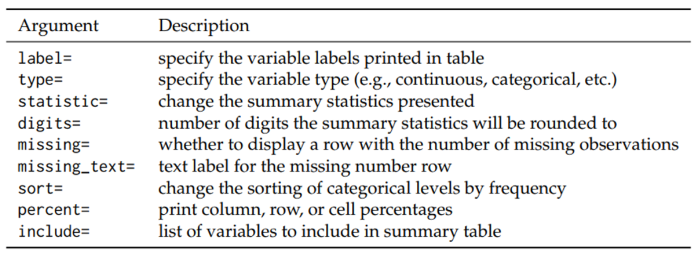
\includegraphics[width=9.72in]{../img/res_1_} \end{figure}
\item
  \textbf{add\ldots()}

  \begin{figure}
  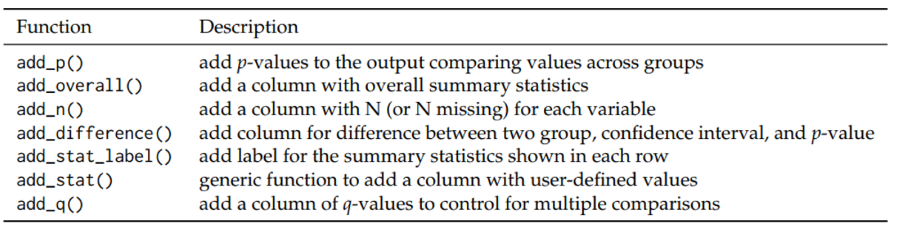
\includegraphics[width=12.5in]{../img/res_2_} \end{figure}
\item
  \textbf{format tableau}

  \begin{figure}
  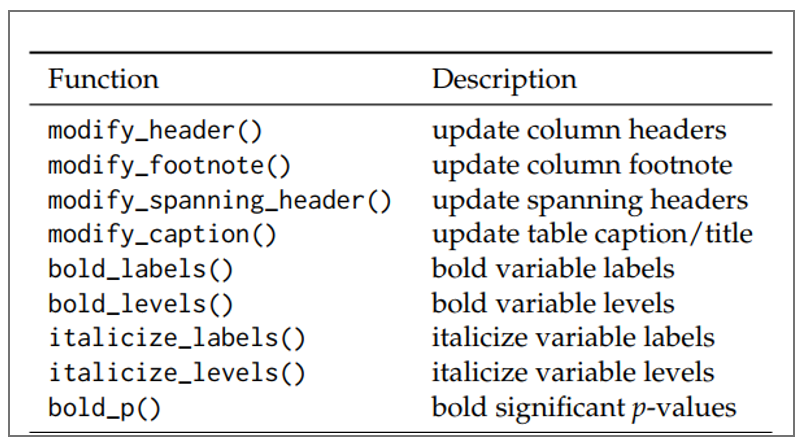
\includegraphics[width=11.1in]{../img/res_3} \end{figure}
\item
  \textbf{Exportation} : gtsave , flextable::save\_as\_docx Les
  principaux tableaux sortis sont dans le fichier \textbf{tableaux\_} du
  dossier \textbf{output}. Vous pouvez vous y référer pour les tableaux
  débordant ou également au fichier html.
\end{itemize}

\newpage

\hypertarget{vi-bibliographie-et-webographie}{%
\section{VI Bibliographie et
webographie}\label{vi-bibliographie-et-webographie}}

\begin{itemize}
\item
  \emph{\url{https://www.danieldsjoberg.com/gtsummary-weill-cornell-presentation/\#59}}
\item
  \emph{\url{https://github.com/ddsjoberg/gtsummary}}
\item
  \emph{\url{https://www.danieldsjoberg.com/gtsummary/}}
\item
  \emph{Reproducible Summary Tables with the gtsummary Package by Daniel
  D. Sjoberg, Karissa Whiting, Michael Curry, Jessica A. Lavery, Joseph
  Larmarange}
\item
  \emph{\url{https://larmarange.github.io/analyse-R/gtsummary.html}}
\end{itemize}

\end{document}
